\chapter{Theoretical introduction}
	
\section{Problem introduction}

The general task is to predict a weather state $\Omega^t$, observed at a time $t$, given $s$ past timestamps, which are essentially previous weather states: $(\Omega^{t-s \Delta d}, ..., \Omega^{t-\Delta d})=\Omega^{(t-s\Delta d):(t-\Delta t)}$, where $\Delta d$ is the step length, in our examination arbitrarily chosen to be equal to 6 hours. For simplicity in further considerations we will use $\Omega^{t\pm1}$ instead of $\Omega^{t\pm\Delta d}$. We denote weather state at a timestamp $t$ as a tensor of a shape: (latitude span, longitude span, features), therefore our complete input data as well as prediction would be 4-dimensional tensors with an additional dimension for a time \footnote{For neural network based solutions it will be 5-dimensional due to the usage of batches.} \footnote{Additional dimension occurs when using neighbor extension \ref{chap:neighbors}.}. Spatial span was selected so as to cover the border of the entirety of Poland and some of its neighbouring territories. More details regarding data are discussed in chapter \ref{chap:dataset}. High-level spatio-temporal prediction framework is presented at Figure \ref{fig:in_out}

Forecasting performance would be evaluated by the objective functions known as \emph{mean absolute error} and \emph{root mean squared error}, defined, respectively, as: 
\begin{flalign*}
    \mathcal{L}_{MAE}(\hat{\mathbf{Y}}, \mathbf{Y}) &= \frac{1}{n} \sum_{i=1}^{n} |y_i - \hat{y}_i| \\ \\
    \mathcal{L}_{RMSE}(\hat{\mathbf{Y}}, \mathbf{Y}) &= \sqrt{\frac{1}{n} \sum_{i=1}^{n} (y_i - \hat{y}_i)^2}
\end{flalign*}
\noindent where $\hat{\mathbf{Y}}$ is the tensor of predictions and $\mathbf{Y}$ is the tensor of ground truth values. The application of these functions will be separated into two situations:
\begin{itemize}
    \item They will be computed for all features separately to obtain interpretable results regarding prediction performance related to a given feature.
    \item In neural networks loss function calculation and for the analysis presented in Chapter \ref{chap:report}, they will be computed on the normalized version of features, resulting in a more abstract but singular score.
\end{itemize}

\subsection{Naming convention}
 For further convenience, we propose a general naming convention presented in \ref{tab:name_conv} and \ref{tab:model_conv}. 
 \begin{table}[!ht]
    \centering
     \begin{tabular}{|c|c|}
        \hline
        Symbol & Description \\
        \hline
        $\mathbf{f}$ & Set of features: $(f_1,..., f_n)$ \\
        $s$ & Number of past steps \\
        $h$ & Forecasting horizon \\
        $\Omega$ & Real weather state for all features \\
        $\mathbf{X}$ & Input weather state tensor  \\
        $\mathbf{Y}$ & Target weather state tensor  \\
        $\hat{\mathbf{Y}}$ & Predicted weather state tensor \\
        $\mathbf{x}$ & Input weather state at a single grid box \\
        $\mathbf{y}$ & Target weather state at a single grid box \\
        $\hat{\mathbf{y}}$ & Predicted weather state at a single grid box \\
        \hline
    \end{tabular}
    \caption{General conventions}
    \label{tab:name_conv}
 \end{table}

Additionally, for each weather tensor $(\mathbf{X}, \mathbf{Y}, \hat{\mathbf{Y}})$, the superscript represents time-related information, signifying the state at a given timestamp (e.g., $\mathbf{X}^t$), or a set of states from $t$ to $t'$ timestamps inclusively (e.g., $\mathbf{X}^{t:t'}$). The subscript indicates the specific feature to which the tensor applies (e.g., $\mathbf{X}_{f_j}$). A tensor with no subscripts by default applies to all features: for $\mathbf{X}$, to all $s$ past steps, and for $\mathbf{Y}$ and $\hat{\mathbf{Y}}$, to all $h$ future steps. We also highlight lowercase letters $(\mathbf{x},\mathbf{y},\hat{\mathbf{y}})$ representing the weather state for a single grid box.
 
\begin{table}[!ht]
    \centering
    \begin{tabular}{|c|c|c|}
        \hline
        Model Notation & Abbreviation & Model Description \\
        \hline
        $\Phi^{ES}$  & $ES$ & Exponential Smoothing \\
        $\Phi^{SLR}$ & $SLR$ & Simple Linear Regression \\
        $\Phi^{LR}$  & $LR$ & Linear Regression \\
        $\Phi^{GB}$ & $GB$ & Gradient Boosting Trees \\
        \hline
    \end{tabular}
\caption{Baseline model conventions}
\label{tab:model_conv}
\end{table}
 
 It is crucial to emphasize the fact that the scale of values of distinct features is diverse. Therefore, we define a model $\Phi$ as a collection of independent sub-models, each exclusively responsible for predicting distinct feature $f_j$. This solution was proposed to avoid situations in which the statistical dispersion of one feature might influence the prediction of another feature.  
 \[
 \Phi = (\Phi_{f_1}, ..., \Phi_{f_n})
 \]
  In further considerations, we will use a term: sub-models for each of $\Phi_{f_j}$. This is not applied to neural network solutions \ref{NN-theory}, which always use the singular model to predict all target features simultaneously.

\subsection{General prediction framework}

\begin{figure}[!h]

\tikzset{every picture/.style={line width=0.75pt}} %set default line width to 0.75pt        

\begin{tikzpicture}[x=0.75pt,y=0.75pt,yscale=-1,xscale=1]
%uncomment if require: \path (0,389); %set diagram left start at 0, and has height of 389

%Shape: Cube [id:dp2816308175879604] 
\draw   (58.25,114.54) -- (81.78,91.01) -- (137.08,91.01) -- (137.08,145.91) -- (113.55,169.44) -- (58.25,169.44) -- cycle ; \draw   (137.08,91.01) -- (113.55,114.54) -- (58.25,114.54) ; \draw   (113.55,114.54) -- (113.55,169.44) ;
%Shape: Brace [id:dp4309828249836092] 
\draw   (76.63,89.37) .. controls (73.72,86.74) and (70.94,86.88) .. (68.31,89.8) -- (68.31,89.8) .. controls (64.55,93.97) and (61.21,94.73) .. (58.29,92.1) .. controls (61.21,94.73) and (60.79,98.13) .. (57.03,102.29)(58.72,100.42) -- (57.03,102.29) .. controls (54.4,105.21) and (54.54,107.99) .. (57.45,110.62) ;
%Shape: Brace [id:dp7756675475750493] 
\draw   (51.06,119.6) .. controls (46.39,119.75) and (44.14,122.16) .. (44.29,126.83) -- (44.53,134.35) .. controls (44.75,141.01) and (42.53,144.42) .. (37.86,144.57) .. controls (42.53,144.42) and (44.97,147.67) .. (45.19,154.34)(45.09,151.34) -- (45.43,161.86) .. controls (45.58,166.52) and (47.99,168.77) .. (52.66,168.62) ;
%Shape: Brace [id:dp612063156099937] 
\draw   (60.65,174.34) .. controls (60.72,179.01) and (63.09,181.3) .. (67.76,181.23) -- (76.73,181.09) .. controls (83.4,180.98) and (86.77,183.26) .. (86.84,187.93) .. controls (86.77,183.26) and (90.06,180.88) .. (96.73,180.78)(93.73,180.82) -- (105.71,180.64) .. controls (110.38,180.57) and (112.67,178.2) .. (112.6,173.53) ;
%Shape: Cube [id:dp42835259632452516] 
\draw   (201.31,112.9) -- (224.84,89.37) -- (280.14,89.37) -- (280.14,144.28) -- (256.61,167.81) -- (201.31,167.81) -- cycle ; \draw   (280.14,89.37) -- (256.61,112.9) -- (201.31,112.9) ; \draw   (256.61,112.9) -- (256.61,167.81) ;
%Shape: Brace [id:dp07592439753840141] 
\draw   (89.33,238.35) .. controls (89.33,243.02) and (91.66,245.35) .. (96.33,245.35) -- (149.81,245.35) .. controls (156.48,245.35) and (159.81,247.68) .. (159.81,252.35) .. controls (159.81,247.68) and (163.14,245.35) .. (169.81,245.35)(166.81,245.35) -- (223.29,245.35) .. controls (227.96,245.35) and (230.29,243.02) .. (230.29,238.35) ;
%Shape: Cube [id:dp7110500253196546] 
\draw   (376.35,113.72) -- (399.88,90.19) -- (455.18,90.19) -- (455.18,145.09) -- (431.65,168.62) -- (376.35,168.62) -- cycle ; \draw   (455.18,90.19) -- (431.65,113.72) -- (376.35,113.72) ; \draw   (431.65,113.72) -- (431.65,168.62) ;
%Shape: Brace [id:dp86120893233015] 
\draw   (392.33,90.19) .. controls (389.42,87.56) and (386.64,87.7) .. (384.01,90.62) -- (384.01,90.62) .. controls (380.25,94.78) and (376.91,95.54) .. (373.99,92.91) .. controls (376.91,95.54) and (376.49,98.94) .. (372.73,103.11)(374.42,101.24) -- (372.73,103.11) .. controls (370.1,106.02) and (370.24,108.8) .. (373.15,111.43) ;
%Shape: Brace [id:dp9673653209625941] 
\draw   (369.15,118.79) .. controls (364.49,118.94) and (362.24,121.34) .. (362.39,126.01) -- (362.63,133.53) .. controls (362.85,140.2) and (360.63,143.6) .. (355.96,143.75) .. controls (360.63,143.6) and (363.07,146.86) .. (363.28,153.52)(363.19,150.52) -- (363.53,161.04) .. controls (363.68,165.71) and (366.09,167.96) .. (370.75,167.81) ;
%Shape: Brace [id:dp9113296386668477] 
\draw   (378.74,173.53) .. controls (378.81,178.2) and (381.18,180.49) .. (385.85,180.42) -- (394.83,180.27) .. controls (401.5,180.17) and (404.87,182.45) .. (404.94,187.12) .. controls (404.87,182.45) and (408.16,180.07) .. (414.83,179.96)(411.83,180.01) -- (423.8,179.82) .. controls (428.47,179.75) and (430.76,177.38) .. (430.69,172.71) ;
%Shape: Cube [id:dp35039842919754816] 
\draw   (521.31,112.9) -- (544.84,89.37) -- (600.14,89.37) -- (600.14,144.28) -- (576.61,167.81) -- (521.31,167.81) -- cycle ; \draw   (600.14,89.37) -- (576.61,112.9) -- (521.31,112.9) ; \draw   (576.61,112.9) -- (576.61,167.81) ;
%Shape: Brace [id:dp3763157845274283] 
\draw   (407.33,239.35) .. controls (407.33,244.02) and (409.66,246.35) .. (414.33,246.35) -- (467.81,246.35) .. controls (474.48,246.35) and (477.81,248.68) .. (477.81,253.35) .. controls (477.81,248.68) and (481.14,246.35) .. (487.81,246.35)(484.81,246.35) -- (541.29,246.35) .. controls (545.96,246.35) and (548.29,244.02) .. (548.29,239.35) ;

% Text Node
\draw (33.24,96.31) node [anchor=north west][inner sep=0.75pt]  [rotate=-309.39,xslant=-0.03] [align=left] {{\scriptsize features}};
% Text Node
\draw (79.43,212.59) node [anchor=north west][inner sep=0.75pt]    {$X_{t}$};
% Text Node
\draw (167.65,116.51) node [anchor=north west][inner sep=0.75pt]   [align=left] {...};
% Text Node
\draw (21.86,173.65) node [anchor=north west][inner sep=0.75pt]  [rotate=-270.99] [align=left] {{\scriptsize latitude span}};
% Text Node
\draw (52.73,186.5) node [anchor=north west][inner sep=0.75pt]   [align=left] {{\scriptsize longitude span}};
% Text Node
\draw (209.49,210.96) node [anchor=north west][inner sep=0.75pt]    {$X_{t+s-1}$};
% Text Node
\draw (171.04,208.29) node [anchor=north west][inner sep=0.75pt]   [align=left] {...};
% Text Node
\draw (153.16,258.53) node [anchor=north west][inner sep=0.75pt]    {$\mathbf{X}$};
% Text Node
\draw (433.72,32.89) node [anchor=north west][inner sep=0.75pt]   [align=left] {{\Large Model Output}};
% Text Node
\draw (108.05,32.26) node [anchor=north west][inner sep=0.75pt]   [align=left] {{\Large Model Input}};
% Text Node
\draw (348.14,97.12) node [anchor=north west][inner sep=0.75pt]  [rotate=-309.39,xslant=-0.03] [align=left] {{\scriptsize features}};
% Text Node
\draw (339.95,172.84) node [anchor=north west][inner sep=0.75pt]  [rotate=-270.99] [align=left] {{\scriptsize latitude span}};
% Text Node
\draw (369.83,186.68) node [anchor=north west][inner sep=0.75pt]   [align=left] {{\scriptsize longitude span}};
% Text Node
\draw (487.65,116.51) node [anchor=north west][inner sep=0.75pt]   [align=left] {...};
% Text Node
\draw (396.43,207.59) node [anchor=north west][inner sep=0.75pt]    {$\hat{Y}_{t+s}$};
% Text Node
\draw (525.49,206.96) node [anchor=north west][inner sep=0.75pt]    {$\hat{Y}_{t+s+fh-1}$};
% Text Node
\draw (488.04,209.29) node [anchor=north west][inner sep=0.75pt]   [align=left] {...};
% Text Node
\draw (471.16,259.53) node [anchor=north west][inner sep=0.75pt]    {$\hat{\mathbf{Y}}$};


\end{tikzpicture}


\label{fig:in_out} \caption{Spatio-Temporal prediction framework} 

\end{figure}


The general framework of prediction is as follows: taking as input the past $s$ weather states $\mathbf{X}^{(t-s+1):(t)}=\mathbf{X}$, the models output the predicted next $h$ weather states $\hat{\mathbf{Y}}^{(t+1):(t+h)}=\hat{\mathbf{Y}}$. \\

It is worth taking into account the fact that this framework may differ when applying techniques such as grid neighbors \ref{chap:neighbors} or using constant encoding \ref{chap:feat_eng}. Details regarding those differences are explained deeply in subsequent chapters.


\section{Explored techniques}
 \subsection{Autoregression}
 Each baseline model is designed to forecast the entire weather state for the subsequent timestamp, with the forecasting horizon set at one. Therefore, when employing our models for short-term prediction tasks exceeding a few timestamps into the future, the autoregressive approach could be used. \\

 We denote model input as $\mathbf{X}$ and model output as $\hat{\mathbf{Y}}$ according to the convention in \ref{tab:name_conv} and $\oplus$ operation as concatenation of tensors. With assumption that $h \le s$, autoregression is $h$-steps prediction process such that:
 \begin{flalign*}
    &\hat{\mathbf{Y}}^{t+1} = \Phi(\mathbf{X}^{(t-s+1):(t)}) \\
    &\hat{\mathbf{Y}}^{t+2} = \Phi(\mathbf{X}^{(t-s+2):(t)} \oplus \hat{\mathbf{Y}}^{t+1}) \\
    &\hat{\mathbf{Y}}^{t+3} = \Phi(\mathbf{X}^{(t-s+3):(t)} \oplus \hat{\mathbf{Y}}^{(t+1):(t+2)}) \\
    &\vdots \\
    &\hat{\mathbf{Y}}^{t+h} = \Phi(\mathbf{X}^{(t-s+h):(t)} \oplus \hat{\mathbf{Y}}^{(t+1):(t+h-1)})
 \end{flalign*}

 Therefore, by simplifying:
 \[
    \hat{\mathbf{Y}} = \Phi(\mathbf{X})
 \]
 
 For each model except $\Phi^{slr}$, during every autoregressive step concatenation of outputs from sub-models is required, whereas $\mathbf{X}^t$ needs to have information from every feature:
 \begin{flalign*}
    &\hat{\mathbf{Y}}^{t+1}_{f_j} = \Phi_{f_j}(\mathbf{X}^{t}) \\
    &\hat{\mathbf{Y}}^{t+1} = \hat{\mathbf{Y}}^{t+1}_{f_1} \oplus \ldots \oplus \hat{\mathbf{Y}}^{t+1}_{f_n}
 \end{flalign*}

\subsection{Neighbors Extension}\label{chap:neighbors}
For every input tensor we have implemented an extension called additional neighbors. It expands all data points to include information from closely located grid boxes. Selection of neighbours is determined by the relative distance (radius) between the center of grid-boxes: $r$. In the Figure \ref{fig:neighbors}, grey-colored grid boxes represent the primary data point and black boxes represent its neighbors.

\begin{figure}[!ht]
    \centering
    \begin{tikzpicture}[scale=0.5]
        \draw[step=1, black] (0,0) grid (7,7);
        \filldraw[fill=gray, draw=white] (3,3) rectangle (4,4);
        \filldraw[fill=black, draw=white] (3,2) rectangle (4,3);
        \filldraw[fill=black, draw=white] (2,3) rectangle (3,4);
        \filldraw[fill=black, draw=white] (3,4) rectangle (4,5);
        \filldraw[fill=black, draw=white] (4,3) rectangle (5,4);
        
        \begin{scope}[shift={(9,0)}]
            \draw[step=1, black] (0,0) grid (7,7);
            \foreach \i in {1, ..., 9} {
                \pgfmathtruncatemacro\row{mod(\i-1,3)}
                \pgfmathtruncatemacro\col{int((\i-1)/3)}
                \filldraw[fill=black, draw=white] (\row+2,\col+2) rectangle (\row+3,\col+3);
            }
            \filldraw[fill=gray, draw=white] (3,3) rectangle (4,4);
            \filldraw[fill=black, draw=white] (1,3) rectangle (2,4);
            \filldraw[fill=black, draw=white] (5,3) rectangle (6,4);
            \filldraw[fill=black, draw=white] (3,1) rectangle (4,2);
            \filldraw[fill=black, draw=white] (3,5) rectangle (4,6);
        \end{scope}

        \begin{scope}[shift={(18,0)}]
            \draw[step=1, black] (0,0) grid (7,7);
            \foreach \i in {1, ..., 25} {
                \pgfmathtruncatemacro\row{mod(\i-1,5)}
                \pgfmathtruncatemacro\col{int((\i-1)/5)}
                \filldraw[fill=black, draw=white] (\row+1,\col+1) rectangle (\row+2,\col+2);
            }
            \filldraw[fill=gray, draw=white] (3,3) rectangle (4,4); 
            \filldraw[fill=black, draw=white] (0,3) rectangle (1,4);
            \filldraw[fill=black, draw=white] (6,3) rectangle (7,4);
            \filldraw[fill=black, draw=white] (3,0) rectangle (4,1);
            \filldraw[fill=black, draw=white] (3,6) rectangle (4,7);
        \end{scope}
    \end{tikzpicture}
    \caption{Neighbors logic for $r=(1,2,3)$}
    \label{fig:neighbors}
\end{figure}

Below be present formal definition, assuming that grid boxes has resolution (1x1) and according to Table \ref{tab:neigh_conv}:
\renewcommand{\arraystretch}{1.25}
\begin{table}[!ht]
    \centering
    \begin{tabular}{|c|c|}
        \hline
        Symbol & Description \\
        \hline
        $v_{i,j}$ & Grid box at latitude $i$ and longitude $j$ \\
        $\mathcal{V}^G$  & Set of all grid boxes \\
        $\|v_{m,n} - v_{i,j}\|^2$  & Euclidian distance between centres of $v_{m,n}$ and $v_{i,j}$ \\
        $\mathcal{N}(v)$ & Set of neighbors for grid box $v$ \\
        \hline
    \end{tabular}
\caption{Neighbor conventions}
\label{tab:neigh_conv}
\end{table}
\renewcommand{\arraystretch}{1}
\[
    \forall v_{i,j} \in \mathcal{V}^G: \{\forall v_{m,n \neq i,j} : \|v_{m,n} - v_{i,j}\|^2 \le r\} \in \mathcal{N}(v_{i,j})
\]

Unfortunately, the trade-off between memory footprint, computational complexity, and performance gain was not sufficient to incorporate and test bigger $r$ values.

 
 \section{Literature review}
 %distinguishing short-term weather prediction and medium-to-large weather prediction: \cite{app132112019} \\ 
Now that we have stated the problem, we would like to shortly inspect current research and results in the field of MLWP. Therefore, we present a short review of quality papers related to this problem and broadly considered as current state-of-the-art solutions. For a more in-depth exploration of the subject, we recommend referring to the article that inspired our selection of the discussed architectures \cite{app132112019}.

\subsection{GraphCast} \label{sec:graphcast}
\begin{figure}[!ht]
    \centering
    \includegraphics[scale=0.35]{figures/enc_pro_dec.png}
    \caption{Three main components of GraphCast \cite{lam2023graphcast}}
    \label{fig:enc_pro_dec}
\end{figure}

GraphCast was the main inspiration for our work on the weather forecasting problem \cite{lam2023graphcast}. Published in late 2022 by Google Deepmind, was the first MLWP model to notably outperform state-of-the-art NWP methods (HRES) on multiple benchmarks. Furthermore, it is already being incorporated by ECMWF \cite{graphcast-deepmind}. The out-of-the-box approach to solving the problem by constructing a heterogeneous graph divided into 3 components: Encoder, Processor, and Decoder -- Figure \ref{fig:enc_pro_dec}, with a component called Multi Mesh and multiple graph layers aggregating information from neighboring objects proved to be very successful. The architecture itself relies on the graph $\mathcal{G}$, which distinguishes 5 elements:
\begin{itemize}
    \item $\mathcal{V}^{G}$: The set of vertices of the grid,
    \item $\mathcal{V}^M$: The set of multi-mesh vertices,
    \item $\mathcal{E}^{G2M}$: The set of edges from the grid to the multi-mesh,
    \item $\mathcal{E}^{M}$: The set of edges inside the multi-mesh
    \item $\mathcal{E}^{M2G}$: The set of edges from the multi-mesh to the grid
\end{itemize} 

The authors of this solution use 474 input features, all included in $\mathcal{V}^{G}$:
\begin{itemize}
    \item Weather features: 2 timestamps of 5 surface variables and 6 atmospheric variables measured at 37 pressure levels
    \item Constants: 5 static features containing encoded spatial information as well as binary land-sea mask and geopotential
    \item Forcing terms: consist of 5 encoded temporal features for 3 timestamps (one lead timestamp) and also includes analytically computed solar radiation
\end{itemize}

Other components have no weather context. All edges encode only spatial information such as edge lengths and coordinate differences, $\mathcal{V}^M$ encode only latitude and longitude values. The process of transferring weather knowledge to those components is discussed in subsequent subchapters.

\subsubsection{Message-passing} 
The whole essence of graph neural networks is the use of the message-passing algorithm. It is based on the aggregation of information from neighbors (usually neighboring nodes, but it can also be edges if they have features). The aggregation function must be permutation invariant: popular choices are average or sum. Example message-passing step using average function:
\[
    H_i^{t+1} = ReLU\left(H_i^t W  + \frac{1}{|\mathcal{N}(i)|} \sum_{j \in \mathcal{N}(i)} H_j^t U\right)
\]
%\WK{Paranthesis should be adaptable to what is inside using $\backslash$left( and $\backslash$right)}
\begin{table}[!ht]
    \centering
    \begin{tabular}{|c|c|}
        \hline
        Symbol & Description \\
        \hline
        $H_i^t$& Neuron state at $t$ step of algorithm \\
        $W,U$ & Weight tensors \\
        $\mathcal{N}(i)$ & Set of neighbors for neuron $H_i$ \\
        \hline
    \end{tabular}
\end{table}

\subsubsection{Multi-mesh}\label{chap:multi-mesh}
The process of creating a multi-mesh involves iteratively dividing each face of a polyhedron into four parts to increase resolution (Figure \ref{fig:mesh-face}). At first, 12 vertices with uniform resolution are placed across the globe and connected by edges: $M_0$, then there are 6 iterations of the mentioned division, consequently obtaining $M_6$ with more than 40 thousand vertices (Figure \ref{fig:multi-mesh}). All generated polyhedra: $(M_0,..., M_6)$ are connected to form a multi-mesh with multiple edges of different lengths that will later be able to assimilate both short and long-distance weather contexts. \\

\begin{figure}[!ht]
    \centering
    \includegraphics[scale=0.35]{figures/multi_mesh.png}
    \caption{Simultaneous multi-mesh message-passing \cite{lam2023graphcast}}
    \label{fig:multi-mesh}
\end{figure}
\begin{figure}[!ht]
    \centering

\tikzset{every picture/.style={line width=0.75pt}} %set default line width to 0.75pt        
\begin{tikzpicture}[x=0.75pt,y=0.75pt,yscale=-1,xscale=1]
%uncomment if require: \path (0,300); %set diagram left start at 0, and has height of 300

%Shape: Triangle [id:dp5526310537518102] 
\draw   (184.18,86.13) -- (209,113.13) -- (159,113.13) -- cycle ;
%Straight Lines [id:da5309512728134356] 
\draw    (184,113.13) -- (171,100.13) ;
%Straight Lines [id:da318567472926536] 
\draw    (171,100.13) -- (197,100.13) ;
%Straight Lines [id:da5008865323179771] 
\draw    (184,113.13) -- (197,100.13) ;
%Shape: Triangle [id:dp3052310642312507] 
\draw   (94.68,86.63) -- (119.5,113.63) -- (69.5,113.63) -- cycle ;
%Straight Lines [id:da020905912975204166] 
\draw    (125,100.13) -- (147,100.13) ;
\draw [shift={(149,100.13)}, rotate = 180] [color={rgb, 255:red, 0; green, 0; blue, 0 }  ][line width=0.75]    (10.93,-3.29) .. controls (6.95,-1.4) and (3.31,-0.3) .. (0,0) .. controls (3.31,0.3) and (6.95,1.4) .. (10.93,3.29)   ;

\end{tikzpicture}
    \caption{Multi-mesh face division}
    \label{fig:mesh-face}
\end{figure}

\subsubsection{Generation of $\mathcal{E}^{M2G}$ and $\mathcal{E}^{G2M}$}
Considering $\mathcal{V}^{G}$ as input data, having already described the creation process of $\mathcal{V}^M$ and $\mathcal{E}^{M}$, connecting these two graphs requires generation of $\mathcal{E}^{M2G}$ and $\mathcal{E}^{G2M}$. \WK{Expand these symbols here, the reader doesn't want to continuously look into the table where $\mathcal{E}^{G2M}$ is explained **Maciej - I put the table below again**}

Multi-mesh refined space with the lowest resolution denoted as $M_6$ is constructed so that each face of it, specifically all three of the nodes that create such face, might be connected to the nearest grid node.

A reverse connection is generated when the distance between the grid node and mesh node is less or equal to 0.6 lengths of $M_6$ edge:
\[
    d_{v_i^G,v_j^M} \leq 0.6e^{M_6}
\]
It ensures that every grid point is connected with at least one mesh node.

\begin{table}[!ht]
    \centering
    \begin{tabular}{|c|c|}
        \hline
        Symbol & Definition \\
        \hline
        $\mathcal{V}^{G}$ & Set of vertices of the grid \\
        $\mathcal{V}^M$ & Set of multi-mesh vertices \\
        $\mathcal{E}^{G2M}$ & Set of edges from the grid to the multi-mesh \\
        $\mathcal{E}^{M}$ & Set of edges inside the multi-mesh \\
        $\mathcal{E}^{M2G}$ & Set of edges from the multi-mesh to the grid \\
        \hline 
    \end{tabular}
    \caption{Symbols and their definition}
    \label{tab:graphcast-symbols}
\end{table}

\subsubsection{Encoder} 
At the very beginning, all graph components go through MLP layers to obtain the same latent space dimension for later convenience of information aggregation at the message-passing step. Then a single GNN layer is applied to pass weather information to the multi-mesh, updating the edge representations $\mathcal{E}^{G2M}$ by aggregating information from adjacent nodes, and updating the node representations $\mathcal{V}^M$ by aggregating all the already updated edges arriving into a particular mesh node. In addition, residual connections are applied to all components involved in this part of the algorithm.
 % \begin{flalign*}
 %    &\mathcal{V}^{G} = MLP(\mathcal{V}^{G}) \\
 %    &\mathcal{V}^M = MLP(\mathcal{V}^M) \\
 %    &\mathcal{E}^{G2M} = MLP(\mathcal{E}^{G2M}) \\
 %    &\mathcal{E}^{M} = MLP(\mathcal{E}^{M}) \\
 %    &\mathcal{E}^{M2G} = MLP(\mathcal{E}^{M2G}) \\
 % \end{flalign*}

\subsubsection{Processor}
The message-passing algorithm runs similarly as in the Encoder, first updating the $\mathcal{E}^M$ and then $\mathcal{V}^M$. Finally, residual connections are added identically as before. This process is performed iteratively 16 times, with each iteration expanding and enriching the weather context for all multi-mesh components.

\subsubsection{Decoder}
To return to the grid and the target representation of the weather state, another graph layer is applied. It updates $\mathcal{E}^{M2G}$ and $\mathcal{V}^G$ sequentially, along with the residual connections. Finally, a final MLP layer is added to change the hidden dimension to match the number of target features. 

It is worth noting that the model does not predict the next state of the weather, but the difference between the state of the previous state and the predicted state:
\[
    \hat{\mathbf{Y}}^{t+1} = \text{GraphCast}(\mathbf{X}^{t':t}) + \mathbf{X}^t
\]
In addition, the cost function is calculated autoregressively and the forecasting horizon increases sequentially with training progress.
% \[
%     \mathcal{L}(\hat{\mathbf{X}}^{t':t} \oplus \hat{\mathbf{Y}}^{t:t''}, \mathbf{Y}^{t:t''})
% \]
% **not sure if formula needed nor correct though.

\subsection{MetNet}
\begin{figure}
    \centering
    \includegraphics[scale=0.6]{figures/MetNet.png}
    \caption{MetNet architecture overview \cite{DBLP:journals/corr/abs-2003-12140}}
    \label{fig:metnet}
\end{figure}
Another notable architecture is MetNet, proposed by Google Research \cite{DBLP:journals/corr/abs-2003-12140}. It primarily aims to leverage the strengths of both convolutional and recurrent neural networks for spatio-temporal data. Its substantial difference from the GraphCast architecture is that it works on patches of the Earth instead of the entire globe: (1024 $\times$ 1024) km grid. Moreover, the frequency of the considered weather states is eminently high: 15-minute time steps. Architecture is divided into 3 components:
\subsubsection{Spatial Downsampler}
The component that works independently on the spatial dimension. Its task is to work as an encoder to create more compact latent space by obtaining multiple convolutional and max pooling operations that aggregate and encode spatial features of data.
\subsubsection{Temporal Encoder}
As its name suggests it focuses on temporal dimension working parallel to Spatial Downsampler. It leverages Convolutional Long Short-Term Memory (ConvLSTM) layers that capture the temporal context of data, emphasizing the influence of the most recent timestamps in the input tensors \cite{shi2015convolutional}. 
\subsubsection{Spatial Aggregator}
The last component functions as a robust decoder. Instead of a classic multilayer perceptron, MetNet incorporates axial self-attentive blocks, that enable covering global context within a patch \cite{ho2019axial}.

 An engaging strategy incorporated for the precipitation forecasting problem addressed in a paper published in 2020, is discretizing variables into small intervals and solving a multi-label classification task instead of a regression problem. The motivation behind such an approach is that authors assert that the categorical distribution of data stabilizes their training process. 

\begin{figure}[!ht]
    \centering
    \includegraphics[scale=0.45]{figures/fourcastnet.png}
    \caption{FourCastNet architecture \cite{pathak2022fourcastnet}}
    \label{fig:fourcastnet}
\end{figure}

\subsection{FourCastNet} \label{sec:fourcastnet}
The last model that we want to refer to is FourCastNet \cite{pathak2022fourcastnet}. The motivation behind leveraging it was the tremendous increase in extreme weather events worldwide in recent years and the desire to introduce a model well-suited to high-resolution data.

\subsubsection{Adaptive Fourier Neural Operator}

What sets it apart from previously presented architectures is the fact that it uses the so-called Adaptive Fourier Neural Operator (AFNO) \cite{guibas2022adaptive}, focusing on combining the Fourier Neural Operator \cite{li2021fourier} with a self-attention mechanism \cite{vaswani2023attention}.
It is built with a vision transformer (ViT) backbone \cite{dosovitskiy2021image} that leverages the tokenization of inputs by a patch embedding layer -- spatial data is converted to a sequence of $P\text{x}P$ patches, then flattened and projected into high dimensional space.
Embedded patches are later passed into a transformer encoder that allows different patches to interact and get some context of each other thanks to the attention mechanism.

Fourier Neural Operators implement global convolution operation that can be interpreted as global token mixing, i.e. channel and spatial mixing. They can model those interactions within Fourier space, therefore mitigating computational complexity. Inside the spatial mixing component presented in Figure \ref{fig:fourcastnet}, tensors are passed through the Fast Fourier Transform (FFT) with frequencies multiplied by kernels and then the Inverse Fast Fourier Transform (IFFT) is performed. The entire process is called a global convolution since multiplication in Fourier space is essentially the same as convolution operation in spatial space. The word "Adaptive" in Fourier Neural Operators mainly refers to adjusting the computational complexity even further by:
\begin{itemize}
    \item splitting a kernels into several separate blocks,
    \item using shared weights by each input token, which significantly reduces the number of model parameters
\end{itemize}

%Considering that spatial data in Fourier space is focused mainly on low frequencies, a sparse prior was introduced, which can be used to calculate MAE loss by so-called soft thresholding. 
Channel Mixing is a simple multilayer perceptron that mixes spatial data in the channel dimension.

\subsubsection{Architecture}
The architecture itself consists of 12 AFNO blocks and a Linear Decoder that changes the hidden dimension to match the number of predicted features. In addition, in the research paper, they presented a division into:
\begin{itemize}
    \item pre-training: which is a simple training that predicts single step into the future,
    \item fine-tuning: which calculates cost functions and performs backpropagation with autoregressive prediction taken into account
\end{itemize}

Total precipitation is reportedly extremely challenging to predict having highly sparse features and very different distribution than other features. Therefore they use it as a diagnostic variable and train it on a separate model, which uses AFNO as a backbone.

\subsubsection{Additional information}
The proposed solution is also extremely efficient in terms of computational time due to the usage of different parallelization strategies such as feature parallelism and spatial parallelism. The architecture achieves great results especially in predicting surface winds and hurricane intensity and paths, obtaining results similar to the IFS \cite{ECMWFIFS} for short-term predictions. The proposed approach to the prediction of a very difficult feature of precipitation proved to be very good because the model obtains very satisfactory results in this area as well.

\subsection{Conclusions}
All proposed solutions exhibit both similarities and distinctions. We drew inspiration from some of these approaches and incorporated them into our model extensively described in Chapter \ref{chap:model}. Each model focuses on 3 main aspects, crucial in the task of weather prediction and in the whole field of working with spatio-temporal data:
\begin{enumerate}[a)]
    \item \textbf{Creating an abstract representation of the weather state through embeddings or downsampling}: GraphCast uses $MLP^{Embedder}$ and multi-mesh representation, MetNet includes a spatial downsampler while FourCastNet incorporates AFNO and creates patch embeddings,
    \item \textbf{Dealing with temporal features}: both MetNet and FourCastNet make use of attention mechanisms, which in recent years achieved outstanding results for all problems dealing with sequentially-structured data, the former additionally introduces recursive ConvLSTM layers, while the latter, like GraphCast, introduce fine tuning with calculations of cost functions in an autoregressive manner,
    \item \textbf{Capturing spatial relationships}: leveraging strengths of visual transformer backbone in FourCastNet and making use of classic convolutional networks for MetNet.
\end{enumerate}

The fact of using graph neural networks in GraphCast as a tool to deal with spatio-temporal data and consequently with both points b) and c) was the main inspiration for starting work on our graph model \ref{chap:model}.

 \section{Baselines}\label{chap:baselines}
%  \subsection{Dummy Regression}
% The most primitive baseline always returns a mean value calculated on the train set for each data pixel and feature.
%  \[
%     \hat{\mathbf{Y}} = \overline{\mathbf{Y}}_{train}
%  \]
% I think it will be better to just make a footnote when presenting results than creating entire subchapter for this method.

 \subsection{Exponential Smoothing}
 The first baseline we explored was exponential smoothing -- a method of smoothing time series data using the exponential window function. It was first described by Robert Goodell Brown in 1956 \cite{brown1956exponential} and we are adapting the implementation from the Python library statsmodels \cite{seabold2010statsmodels}. 
 Time series' are sequences of data points, which means in order to use this method, we had to consider our data as an array of time series. To be precise, for every grid box, we had a series of length $s$ for each feature. When predicting, we need to fit the model for each point on the grid and each feature separately. This causes the method to be very slow during prediction when compared to other baselines. Therefore, it is entirely excluded from analysis in Chapter \ref{chap:report}. The formula for predicting the next state is as follows:
 \begin{flalign*}
     &\forall f_i \in \mathbf{f}: \hat{y}^{t+1}_{f_i} = \sum_{j=0}^{s-1}\left( \alpha_{f_i} (1-\alpha_{f_i})^j x^{t-j}_{f_i}\right) + (1-\alpha)^t l_{f_i}
 \end{flalign*}
 \noindent where $\alpha_{f_i}$ is the smoothing coefficient and $l_{f_i}$ is the initial fitted value. Both these values are set independently for each value. Here $\mathbf{x}^{t}_{f_i}$ denotes the value of a single grid box from $\mathbf{X}^{t}_{f_i}$.   
 \WK{This equation does not carry too much information. Write some more about what is actually exponential smoothing -- it is very simple!}
 
 \subsection{Simple Linear Regression}\label{chap:slinear}
 This method is essentially a basic linear regression. When predicting a particular feature $f_i$, each sub-model only considers that specific feature in the input. It is a straightforward approach that assumes no correlation between different features and like any linear regression, it follows the basic assumptions of: linearity, independence, homoscedasticity, normality, absence of multicollinearity, and absence of endogeneity \cite{linear-regression-assumptions}. Given that our task clearly deviates from meeting most of the mentioned assumptions, this method yields results that can be considered fairly average. The entire straightforward mechanism of this method consists of taking as input $s$ past weather states and using the Ordinary Least Squares (OLS) algorithm to find the best linear function of those past weather values that fits our data and, as a result, obtain a forecast for the next future timestamp. As mentioned earlier, each of the sub-models in this method performs completely independently -- to forecast at time $t+1$ each feature $f_i$ belonging to the set of features under consideration $\mathbf{f}$, the model responsible for predicting it takes as input $s$ previous weather states with information only about that feature: $\mathbf{X}^{(t-s+1):(t)}_{f_i}$. To obtain the global predicted weather state at time $t+1$, we need to concatenate the outputs of all the sub-models resulting in a global prediction $\hat{\mathbf{Y}}^{t+1}$.
% \[
%     \forall f_i \in \mathbf{f}: \hat{\mathbf{Y}}^{t+1}_{f_i} = \Phi^{SLR}_{f_i}\left(\mathbf{X}^{(t-s+1):(t)}_{f_i}\right) 
% \]

Each grid box prediction can be interpreted as a linear function, as well as the entire weather state forecast for the given feature:
\begin{flalign*}
    &\forall f_i \in \mathbf{f}: \hat{y}^{t+1}_{f_i} = b + \sum_{j=0}^{s-1} b_j x^{t-j}_{f_i} \\
   % &\forall f_i \in \mathbf{f}: \hat{\mathbf{Y}}^{t+1}_{f_i} = \boldsymbol{\beta_0} + \boldsymbol{\beta}\mathbf{X}^{(t-s+1):(t)}_{f_i} \\
    &\forall f_i \in \mathbf{f}: \hat{\mathbf{Y}}^{t+1}_{f_i} = \boldsymbol{\beta} + \sum_{j=0}^{s-1}\boldsymbol{\beta_j}\mathbf{X}^{t-j}_{f_i}
\end{flalign*}
% This simple model predicting the value of feature $f_i$ at time $t$ as a linear function of its values at previous $s$ times.
\WK{The same situation-- this equation does not tell much. Write in simple words what the model is: predicting the value of feature $f_i$ at time $t$ as a linear function of its values at previous $s$ times.}

 \subsection{Linear Regression}\label{chap:linear}
It follows the same assumptions as \ref{chap:slinear}, but with a tweak. When forecasting the $f_i$ feature, it considers the complete weather state by using all available features as input. This indicate an assumption that different weather features might influence each other. While this approach is still a naive linear model, it leads to slightly improved results. 

The enhanced mechanism proceeds in a manner analogous to its simpler version. Utilizing $s$ past weather states, the OLS algorithm establishes an optimal linear function to predict future weather state from the input data. Each sub-model predicts future weather state at time $t+1$ based on sequences of past weather states containing all available features -- $\mathbf{X}^{(t-s+1):(t)}$. Similarly, to obtain global prediction $\hat{\mathbf{Y}}^{t+1}$, concatenation from sub-models output needs to be performed.
% \[
%     \forall f_i \in \mathbf{f}: \hat{\mathbf{Y}}^{t+1}_{f_i} = \Phi^{LR}_{f_i}\left(\mathbf{X}^{(t-s+1):(t)}\right) 
% \]
Again it allows us to present both grid box and global prediction as a linear function:
 \begin{flalign*}
      &\forall f_i \in \mathbf{f}: \hat{y}^{t+1}_{f_i} = b + \sum_{j=0}^{s-1} \boldsymbol{b}_j \mathbf{x}^{t-j} \\
     % &\forall f_i \in \mathbf{f}: \hat{\mathbf{Y}}^{t+1}_{f_i} = \boldsymbol{\beta_0} + \boldsymbol{\beta}\mathbf{X}^{(t-s+1):(t)}
     &\forall f_i \in \mathbf{f}: \hat{\mathbf{Y}}^{t+1}_{f_i} = \boldsymbol{\beta} + \sum_{j=0}^{s-1}\boldsymbol{\beta_j}\mathbf{X}^{t-j}
 \end{flalign*}
For both \ref{chap:slinear} and \ref{chap:linear}, we have examined the performance of basic linear regression, as well as regularized versions: ridge, lasso, and elastic net (Table \ref{tab:linear-variations}). The outcomes indicate that ridge regression notably outperforms other methods. Further details are provided in Chapter \ref{chap:report}.
\begin{table}[!ht]
    \centering
    \begin{tabular}{|c|c|c|}
        \hline
        Method & Loss Function & Regularization term \\
        \hline
        Linear & $\sum\limits_{i}(y_i - \hat{y_i})^2$  & $\varnothing$ \\
        Ridge & $\sum\limits_{i}(y_i - \hat{y_i})^2$  & $\lambda \sum\limits_{j} b_j^2$ \\
        Lasso & $\sum\limits_{i}(y_i - \hat{y_i})^2$ & $\lambda \sum\limits_{j} |b_j|$ \\
        Elastic Net & $\sum\limits_{i}(y_i - \hat{y_i})^2$ & $\lambda_1 \sum\limits_{j} b_j^2 + \lambda_2 \sum\limits_{j} |b_j|$  \\
        \hline
    \end{tabular}
    \caption{Examined linear regression variations}
    \label{tab:linear-variations}
\end{table}
\WK{The same}
 
\subsection{Gradient Boosting}
Due to the state-of-the-art performance in various tabular data-related challenges, their widespread popularity, and their ability to model complex data, we resolve to implement and analyze solutions based on gradient boosting algorithms. The fundamental idea behind gradient boosting lies in the iterative construction of multiple decision trees. Using the gradient boosting algorithm, these trees are generated to improve outcomes and create a more refined representation in each successive iteration. 

By creating a so-called ensemble, these methods combine outputs from individual trees to enhance predictive accuracy. Unlike random forests that create trees in parallel, gradient boosting adds weak learners sequentially. Each tree corrects errors of the previous one by minimizing the derivative of the loss function with respect to the previous model's output, manipulating the speed of this process by employing a learning rate $\eta$. Therefore, ensemble $F$ at step $j$ can be represented as: 
\[
    F_j = F_{j-1} + \eta * -\frac{\partial \mathcal{L}}{\partial F_{j-1}}
\]
Each of our sub-models predicts the weather state as a combined prediction of all $N$ weak learners in an ensemble:
\[
     \forall f_i \in \mathbf{f}: \hat{\mathbf{Y}}^{t+1}_{f_i} = \sum_{j=1}^{N}\eta F_j\left(\mathbf{X}^{(t-s+1):(t)}\right)
\]

% Their flexibility is further enhanced by the ability to employ distinct hyperparameters for each tree in the ensemble, allowing for fine-tuning and adaptability to diverse aspects of the data.

We chose two widely used methods, XGBoost \cite{Chen_2016} and LightGBM \cite{ke2017lightgbm}, both delivering improved results compared to other baseline methods. While both modes share multiple similarities, the primary distinction lies in their tree construction processes: leaf-wise for XGBoost and level-wise for LightGBM.
% \begin{flalign*}
%     &\forall f_i \in \mathbf{f}: \hat{\mathbf{Y}}^{t+1}_{f_i} = \Phi^{GB}_{f_i}\left(\mathbf{X}^{(t-s+1):(t)}\right)
% \end{flalign*}
\WK{There is no information in these descriptions about the use of neighbor nodes and their features. (This is described in another chapter) This section on baselines is way too short. The baselines should actually be described in comparable details than the known methods from the literature overview that you covered in the previous sections}

\subsection{Additional information}
Due to implementation constraints arising from the lack of support for multidimensional regression in the machine learning frameworks we employed, it was necessary to convert our data dimensionality. This process involved transforming it into a 2-dimensional vector for inputs and a 1-dimensional vector for targets and had to be done for both training and evaluation purposes. For this reason, it was crucial to be careful that each input sample was associated with the correct target. 

In the subsequent analysis, we denote the product of latitude and longitude spans as $S$, number of predicted features as $F$ and number of data samples as $N$, additionally we remind that $s$ represented number of input states. The data were transformed in such a way that the last dimension of the input tensor, called by convention the feature dimension, was equal to the product of the number of input states along with the number of predicted features, while the number of samples, latitudes, and longitudes were combined in first dimension -- for both linear regression and gradient boosting trees, each sub-model was fitted/trained on such inputs: $(N*S,s*F)$. The target tensors were transformed for them so that each sub-model would compare and predict the 1-dimensional tensor associated with the feature -- the number of samples and latitudes and longitudes were stored in 1 dimension: $(N*S)$. 
For a simple linear regression, the situation was a bit simpler with an input tensor that had dimensions: $(N*S, s)$ while output: $(N*S)$, due to the lack of need to use other features than the predicted one for every sub-model.

The situation undergoes a slight shift when employing the neighbor extension described in \ref{chap:neighbors}. The dimensionality of our data expanded and we also dealt with the implementation constraints described above using similar feature aggregation techniques. This process is straightforward, given the number of $n$ neighbors, each one may be interpreted as a new set of features of a size $F$, and therefore our input feature dimensions are expanded to $(N*S, s*F*(n+1))$. The product of the number of weather input features and input sequence length is also multiplied by $n+1$ symbolizing the aggregated features for $n$ neighbors and the reference grid box. 

The inverse transformation, which restored the tensor to its original dimensions, was carried out solely for visualization purposes.

\section{Neural Network Models} \label{NN-theory}
\subsection{U-net}\label{chap:unet}
\begin{figure}[!h]
    \centering


\tikzset{every picture/.style={line width=0.75pt}} %set default line width to 0.75pt        

\begin{tikzpicture}[x=0.75pt,y=0.75pt,yscale=-1,xscale=1]
%uncomment if require: \path (0,555); %set diagram left start at 0, and has height of 555

%Shape: Rectangle [id:dp18715874495438933] 
\draw   (23.66,16.7) -- (26.62,16.7) -- (26.62,200.75) -- (23.66,200.75) -- cycle ;
%Shape: Rectangle [id:dp21108175618544378] 
\draw   (38.43,16.7) -- (42.8,16.7) -- (42.8,200.75) -- (38.43,200.75) -- cycle ;
%Shape: Rectangle [id:dp9926647794913771] 
\draw   (54.61,241.3) -- (58.97,241.3) -- (58.97,333.33) -- (54.61,333.33) -- cycle ;
%Shape: Rectangle [id:dp04703844440598337] 
\draw   (69.88,241.3) -- (78.61,241.3) -- (78.61,333.33) -- (69.88,333.33) -- cycle ;
%Straight Lines [id:da13135618245105463] 
\draw [color={rgb, 255:red, 38; green, 21; blue, 153 }  ,draw opacity=1 ]   (57.52,208.54) -- (57.52,219) ;
\draw [shift={(57.52,221)}, rotate = 270] [color={rgb, 255:red, 38; green, 21; blue, 153 }  ,draw opacity=1 ][line width=0.75]    (6.56,-1.97) .. controls (4.17,-0.84) and (1.99,-0.18) .. (0,0) .. controls (1.99,0.18) and (4.17,0.84) .. (6.56,1.97)   ;
%Shape: Rectangle [id:dp05141207090781941] 
\draw   (93.31,376.64) -- (102.04,376.64) -- (102.04,422.65) -- (93.31,422.65) -- cycle ;
%Shape: Rectangle [id:dp7978080816334711] 
\draw   (112.47,377.79) -- (129.92,377.79) -- (129.92,423.8) -- (112.47,423.8) -- cycle ;
%Shape: Rectangle [id:dp6479639029695707] 
\draw   (139.3,379.22) -- (156.75,379.22) -- (156.75,425.23) -- (139.3,425.23) -- cycle ;
%Shape: Rectangle [id:dp3019357955255262] 
\draw   (144.3,466.7) -- (161.75,466.7) -- (161.75,489.77) -- (144.3,489.77) -- cycle ;
%Shape: Rectangle [id:dp15769795665953923] 
\draw   (172.24,466.91) -- (202.78,466.91) -- (202.78,489.97) -- (172.24,489.97) -- cycle ;
%Shape: Rectangle [id:dp6515995363621675] 
\draw   (213.46,466.95) -- (244,466.95) -- (244,490.01) -- (213.46,490.01) -- cycle ;
%Shape: Rectangle [id:dp8944502071739182] 
\draw   (213.32,524.17) -- (243.86,524.17) -- (243.86,535.7) -- (213.32,535.7) -- cycle ;
%Shape: Rectangle [id:dp8561310330751685] 
\draw   (253.78,523.74) -- (308.31,523.74) -- (308.31,535.27) -- (253.78,535.27) -- cycle ;
%Shape: Rectangle [id:dp5055350538856822] 
\draw   (318.67,524.23) -- (373.21,524.23) -- (373.21,535.76) -- (318.67,535.76) -- cycle ;
%Straight Lines [id:da3574281493968309] 
\draw    (27.11,102.41) -- (35.72,102.41) ;
\draw [shift={(37.72,102.41)}, rotate = 180] [color={rgb, 255:red, 0; green, 0; blue, 0 }  ][line width=0.75]    (6.56,-1.97) .. controls (4.17,-0.84) and (1.99,-0.18) .. (0,0) .. controls (1.99,0.18) and (4.17,0.84) .. (6.56,1.97)   ;
%Shape: Rectangle [id:dp016488727952195026] 
\draw   (54.79,16.7) -- (59.16,16.7) -- (59.16,200.75) -- (54.79,200.75) -- cycle ;
%Straight Lines [id:da15247647004345954] 
\draw    (43.47,102.41) -- (52.08,102.41) ;
\draw [shift={(54.08,102.41)}, rotate = 180] [color={rgb, 255:red, 0; green, 0; blue, 0 }  ][line width=0.75]    (6.56,-1.97) .. controls (4.17,-0.84) and (1.99,-0.18) .. (0,0) .. controls (1.99,0.18) and (4.17,0.84) .. (6.56,1.97)   ;
%Straight Lines [id:da8673701767341216] 
\draw    (59.1,284.62) -- (67.72,284.62) ;
\draw [shift={(69.72,284.62)}, rotate = 180] [color={rgb, 255:red, 0; green, 0; blue, 0 }  ][line width=0.75]    (6.56,-1.97) .. controls (4.17,-0.84) and (1.99,-0.18) .. (0,0) .. controls (1.99,0.18) and (4.17,0.84) .. (6.56,1.97)   ;
%Straight Lines [id:da8818182844686407] 
\draw    (79.46,284.21) -- (88.08,284.21) ;
\draw [shift={(90.08,284.21)}, rotate = 180] [color={rgb, 255:red, 0; green, 0; blue, 0 }  ][line width=0.75]    (6.56,-1.97) .. controls (4.17,-0.84) and (1.99,-0.18) .. (0,0) .. controls (1.99,0.18) and (4.17,0.84) .. (6.56,1.97)   ;
%Shape: Rectangle [id:dp7536745340030019] 
\draw   (90.78,241.71) -- (99.51,241.71) -- (99.51,333.74) -- (90.78,333.74) -- cycle ;
%Straight Lines [id:da2082499344791846] 
\draw    (102.25,400.77) -- (110.07,400.77) ;
\draw [shift={(112.07,400.77)}, rotate = 180] [color={rgb, 255:red, 0; green, 0; blue, 0 }  ][line width=0.75]    (6.56,-1.97) .. controls (4.17,-0.84) and (1.99,-0.18) .. (0,0) .. controls (1.99,0.18) and (4.17,0.84) .. (6.56,1.97)   ;
%Straight Lines [id:da6021949046240975] 
\draw    (129.56,401.43) -- (137.37,401.43) ;
\draw [shift={(139.37,401.43)}, rotate = 180] [color={rgb, 255:red, 0; green, 0; blue, 0 }  ][line width=0.75]    (6.56,-1.97) .. controls (4.17,-0.84) and (1.99,-0.18) .. (0,0) .. controls (1.99,0.18) and (4.17,0.84) .. (6.56,1.97)   ;
%Straight Lines [id:da08664251038435522] 
\draw [color={rgb, 255:red, 38; green, 21; blue, 153 }  ,draw opacity=1 ]   (97.33,346.58) -- (97.33,357.03) ;
\draw [shift={(97.33,359.03)}, rotate = 270] [color={rgb, 255:red, 38; green, 21; blue, 153 }  ,draw opacity=1 ][line width=0.75]    (6.56,-1.97) .. controls (4.17,-0.84) and (1.99,-0.18) .. (0,0) .. controls (1.99,0.18) and (4.17,0.84) .. (6.56,1.97)   ;
%Straight Lines [id:da14969863750099377] 
\draw [color={rgb, 255:red, 38; green, 21; blue, 153 }  ,draw opacity=1 ]   (151.32,433.08) -- (151.32,443.54) ;
\draw [shift={(151.32,445.54)}, rotate = 270] [color={rgb, 255:red, 38; green, 21; blue, 153 }  ,draw opacity=1 ][line width=0.75]    (6.56,-1.97) .. controls (4.17,-0.84) and (1.99,-0.18) .. (0,0) .. controls (1.99,0.18) and (4.17,0.84) .. (6.56,1.97)   ;
%Straight Lines [id:da6267408337269913] 
\draw    (162.06,479.09) -- (169.87,479.09) ;
\draw [shift={(171.87,479.09)}, rotate = 180] [color={rgb, 255:red, 0; green, 0; blue, 0 }  ][line width=0.75]    (6.56,-1.97) .. controls (4.17,-0.84) and (1.99,-0.18) .. (0,0) .. controls (1.99,0.18) and (4.17,0.84) .. (6.56,1.97)   ;
%Straight Lines [id:da7106217929965524] 
\draw    (203.18,479.09) -- (210.99,479.09) ;
\draw [shift={(212.99,479.09)}, rotate = 180] [color={rgb, 255:red, 0; green, 0; blue, 0 }  ][line width=0.75]    (6.56,-1.97) .. controls (4.17,-0.84) and (1.99,-0.18) .. (0,0) .. controls (1.99,0.18) and (4.17,0.84) .. (6.56,1.97)   ;
%Straight Lines [id:da7790605040632763] 
\draw [color={rgb, 255:red, 38; green, 21; blue, 153 }  ,draw opacity=1 ]   (228.02,493.7) -- (228.02,504.15) ;
\draw [shift={(228.02,506.15)}, rotate = 270] [color={rgb, 255:red, 38; green, 21; blue, 153 }  ,draw opacity=1 ][line width=0.75]    (6.56,-1.97) .. controls (4.17,-0.84) and (1.99,-0.18) .. (0,0) .. controls (1.99,0.18) and (4.17,0.84) .. (6.56,1.97)   ;
%Straight Lines [id:da5698357539585125] 
\draw    (243.27,529.93) -- (251.09,529.93) ;
\draw [shift={(253.09,529.93)}, rotate = 180] [color={rgb, 255:red, 0; green, 0; blue, 0 }  ][line width=0.75]    (6.56,-1.97) .. controls (4.17,-0.84) and (1.99,-0.18) .. (0,0) .. controls (1.99,0.18) and (4.17,0.84) .. (6.56,1.97)   ;
%Straight Lines [id:da2416473985612968] 
\draw    (308.6,529.44) -- (316.42,529.44) ;
\draw [shift={(318.42,529.44)}, rotate = 180] [color={rgb, 255:red, 0; green, 0; blue, 0 }  ][line width=0.75]    (6.56,-1.97) .. controls (4.17,-0.84) and (1.99,-0.18) .. (0,0) .. controls (1.99,0.18) and (4.17,0.84) .. (6.56,1.97)   ;
%Straight Lines [id:da809363614141596] 
\draw [color={rgb, 255:red, 12; green, 148; blue, 38 }  ,draw opacity=1 ]   (343.63,506.58) -- (343.63,495.88) ;
\draw [shift={(343.63,493.88)}, rotate = 90] [color={rgb, 255:red, 12; green, 148; blue, 38 }  ,draw opacity=1 ][line width=0.75]    (6.56,-1.97) .. controls (4.17,-0.84) and (1.99,-0.18) .. (0,0) .. controls (1.99,0.18) and (4.17,0.84) .. (6.56,1.97)   ;
%Shape: Rectangle [id:dp025026333432921044] 
\draw   (327.98,465.72) -- (358.52,465.72) -- (358.52,488.79) -- (327.98,488.79) -- cycle ;
%Shape: Rectangle [id:dp20926001651772896] 
\draw  [fill={rgb, 255:red, 51; green, 51; blue, 51 }  ,fill opacity=0.28 ] (297.44,465.72) -- (327.98,465.72) -- (327.98,488.79) -- (297.44,488.79) -- cycle ;
%Straight Lines [id:da7562560240527322] 
\draw [color={rgb, 255:red, 51; green, 51; blue, 51 }  ,draw opacity=0.28 ][fill={rgb, 255:red, 51; green, 51; blue, 51 }  ,fill opacity=0.28 ]   (244.04,477.13) -- (262.58,477.13) -- (295.48,477.13) ;
\draw [shift={(297.48,477.13)}, rotate = 180] [color={rgb, 255:red, 51; green, 51; blue, 51 }  ,draw opacity=0.28 ][line width=0.75]    (6.56,-1.97) .. controls (4.17,-0.84) and (1.99,-0.18) .. (0,0) .. controls (1.99,0.18) and (4.17,0.84) .. (6.56,1.97)   ;
%Shape: Rectangle [id:dp8023052514571293] 
\draw   (368.55,465.68) -- (399.09,465.68) -- (399.09,488.75) -- (368.55,488.75) -- cycle ;
%Shape: Rectangle [id:dp25299169957935863] 
\draw   (409.78,465.72) -- (440.32,465.72) -- (440.32,488.79) -- (409.78,488.79) -- cycle ;
%Straight Lines [id:da701424449135518] 
\draw    (358.37,477.87) -- (366.19,477.87) ;
\draw [shift={(368.19,477.87)}, rotate = 180] [color={rgb, 255:red, 0; green, 0; blue, 0 }  ][line width=0.75]    (6.56,-1.97) .. controls (4.17,-0.84) and (1.99,-0.18) .. (0,0) .. controls (1.99,0.18) and (4.17,0.84) .. (6.56,1.97)   ;
%Straight Lines [id:da6156935246607961] 
\draw    (399.49,477.87) -- (407.31,477.87) ;
\draw [shift={(409.31,477.87)}, rotate = 180] [color={rgb, 255:red, 0; green, 0; blue, 0 }  ][line width=0.75]    (6.56,-1.97) .. controls (4.17,-0.84) and (1.99,-0.18) .. (0,0) .. controls (1.99,0.18) and (4.17,0.84) .. (6.56,1.97)   ;
%Straight Lines [id:da346111466933276] 
\draw [color={rgb, 255:red, 12; green, 148; blue, 38 }  ,draw opacity=1 ]   (424.34,444) -- (424.34,433.3) ;
\draw [shift={(424.34,431.3)}, rotate = 90] [color={rgb, 255:red, 12; green, 148; blue, 38 }  ,draw opacity=1 ][line width=0.75]    (6.56,-1.97) .. controls (4.17,-0.84) and (1.99,-0.18) .. (0,0) .. controls (1.99,0.18) and (4.17,0.84) .. (6.56,1.97)   ;
%Shape: Rectangle [id:dp3443649875713195] 
\draw   (415.23,379.22) -- (432.68,379.22) -- (432.68,425.23) -- (415.23,425.23) -- cycle ;
%Shape: Rectangle [id:dp10916547800365461] 
\draw  [fill={rgb, 255:red, 51; green, 51; blue, 51 }  ,fill opacity=0.28 ] (397.78,379.22) -- (415.23,379.22) -- (415.23,425.23) -- (397.78,425.23) -- cycle ;
%Straight Lines [id:da5453720416120884] 
\draw [color={rgb, 255:red, 51; green, 51; blue, 51 }  ,draw opacity=0.28 ][fill={rgb, 255:red, 51; green, 51; blue, 51 }  ,fill opacity=0.28 ]   (155.7,401.06) -- (174.24,401.06) -- (394.76,401.06) ;
\draw [shift={(396.76,401.06)}, rotate = 180] [color={rgb, 255:red, 51; green, 51; blue, 51 }  ,draw opacity=0.28 ][line width=0.75]    (6.56,-1.97) .. controls (4.17,-0.84) and (1.99,-0.18) .. (0,0) .. controls (1.99,0.18) and (4.17,0.84) .. (6.56,1.97)   ;
%Shape: Rectangle [id:dp7039359315516164] 
\draw   (442.93,379.01) -- (460.39,379.01) -- (460.39,425.02) -- (442.93,425.02) -- cycle ;
%Shape: Rectangle [id:dp1812213827058743] 
\draw   (469.76,379.22) -- (487.21,379.22) -- (487.21,425.23) -- (469.76,425.23) -- cycle ;
%Straight Lines [id:da8986979548500146] 
\draw    (432.72,402) -- (440.53,402) ;
\draw [shift={(442.53,402)}, rotate = 180] [color={rgb, 255:red, 0; green, 0; blue, 0 }  ][line width=0.75]    (6.56,-1.97) .. controls (4.17,-0.84) and (1.99,-0.18) .. (0,0) .. controls (1.99,0.18) and (4.17,0.84) .. (6.56,1.97)   ;
%Straight Lines [id:da7559049364738527] 
\draw    (460.02,402.65) -- (467.84,402.65) ;
\draw [shift={(469.84,402.65)}, rotate = 180] [color={rgb, 255:red, 0; green, 0; blue, 0 }  ][line width=0.75]    (6.56,-1.97) .. controls (4.17,-0.84) and (1.99,-0.18) .. (0,0) .. controls (1.99,0.18) and (4.17,0.84) .. (6.56,1.97)   ;
%Straight Lines [id:da3056268493859836] 
\draw [color={rgb, 255:red, 12; green, 148; blue, 38 }  ,draw opacity=1 ]   (477.78,354.43) -- (477.78,343.73) ;
\draw [shift={(477.78,341.73)}, rotate = 90] [color={rgb, 255:red, 12; green, 148; blue, 38 }  ,draw opacity=1 ][line width=0.75]    (6.56,-1.97) .. controls (4.17,-0.84) and (1.99,-0.18) .. (0,0) .. controls (1.99,0.18) and (4.17,0.84) .. (6.56,1.97)   ;
%Shape: Rectangle [id:dp46850395773139786] 
\draw   (473.6,240.49) -- (482.33,240.49) -- (482.33,332.51) -- (473.6,332.51) -- cycle ;
%Shape: Rectangle [id:dp8888671939844691] 
\draw  [fill={rgb, 255:red, 51; green, 51; blue, 51 }  ,fill opacity=0.28 ] (464.87,240.49) -- (473.6,240.49) -- (473.6,332.51) -- (464.87,332.51) -- cycle ;
%Straight Lines [id:da5063749890219842] 
\draw [color={rgb, 255:red, 51; green, 51; blue, 51 }  ,draw opacity=0.28 ][fill={rgb, 255:red, 51; green, 51; blue, 51 }  ,fill opacity=0.28 ]   (100.07,283.27) -- (118.61,283.27) -- (462.38,283.27) ;
\draw [shift={(464.38,283.27)}, rotate = 180] [color={rgb, 255:red, 51; green, 51; blue, 51 }  ,draw opacity=0.28 ][line width=0.75]    (6.56,-1.97) .. controls (4.17,-0.84) and (1.99,-0.18) .. (0,0) .. controls (1.99,0.18) and (4.17,0.84) .. (6.56,1.97)   ;
%Shape: Rectangle [id:dp6907443953904835] 
\draw   (493.05,240.08) -- (501.78,240.08) -- (501.78,332.1) -- (493.05,332.1) -- cycle ;
%Straight Lines [id:da05860511759288356] 
\draw    (482.27,283.39) -- (490.89,283.39) ;
\draw [shift={(492.89,283.39)}, rotate = 180] [color={rgb, 255:red, 0; green, 0; blue, 0 }  ][line width=0.75]    (6.56,-1.97) .. controls (4.17,-0.84) and (1.99,-0.18) .. (0,0) .. controls (1.99,0.18) and (4.17,0.84) .. (6.56,1.97)   ;
%Straight Lines [id:da27728843868290487] 
\draw    (502.63,282.98) -- (511.24,282.98) ;
\draw [shift={(513.24,282.98)}, rotate = 180] [color={rgb, 255:red, 0; green, 0; blue, 0 }  ][line width=0.75]    (6.56,-1.97) .. controls (4.17,-0.84) and (1.99,-0.18) .. (0,0) .. controls (1.99,0.18) and (4.17,0.84) .. (6.56,1.97)   ;
%Shape: Rectangle [id:dp5538472632746805] 
\draw   (513.95,240.49) -- (522.68,240.49) -- (522.68,332.51) -- (513.95,332.51) -- cycle ;
%Straight Lines [id:da7011046510059195] 
\draw [color={rgb, 255:red, 12; green, 148; blue, 38 }  ,draw opacity=1 ]   (519.23,220.69) -- (519.23,209.99) ;
\draw [shift={(519.23,207.99)}, rotate = 90] [color={rgb, 255:red, 12; green, 148; blue, 38 }  ,draw opacity=1 ][line width=0.75]    (6.56,-1.97) .. controls (4.17,-0.84) and (1.99,-0.18) .. (0,0) .. controls (1.99,0.18) and (4.17,0.84) .. (6.56,1.97)   ;
%Shape: Rectangle [id:dp09592051395907786] 
\draw   (518.32,17.93) -- (522.68,17.93) -- (522.68,201.98) -- (518.32,201.98) -- cycle ;
%Shape: Rectangle [id:dp43041739249131417] 
\draw  [fill={rgb, 255:red, 51; green, 51; blue, 51 }  ,fill opacity=0.28 ] (513.95,17.93) -- (518.32,17.93) -- (518.32,201.98) -- (513.95,201.98) -- cycle ;
%Straight Lines [id:da27741997849623545] 
\draw [color={rgb, 255:red, 51; green, 51; blue, 51 }  ,draw opacity=0.28 ][fill={rgb, 255:red, 51; green, 51; blue, 51 }  ,fill opacity=0.28 ]   (59.72,102.9) -- (78.26,102.9) -- (510.45,102.9) ;
\draw [shift={(512.45,102.9)}, rotate = 180] [color={rgb, 255:red, 51; green, 51; blue, 51 }  ,draw opacity=0.28 ][line width=0.75]    (6.56,-1.97) .. controls (4.17,-0.84) and (1.99,-0.18) .. (0,0) .. controls (1.99,0.18) and (4.17,0.84) .. (6.56,1.97)   ;
%Shape: Rectangle [id:dp9383922675689869] 
\draw   (533.59,17.93) -- (537.95,17.93) -- (537.95,201.98) -- (533.59,201.98) -- cycle ;
%Straight Lines [id:da22056170087348537] 
\draw    (522.26,103.63) -- (530.88,103.63) ;
\draw [shift={(532.88,103.63)}, rotate = 180] [color={rgb, 255:red, 0; green, 0; blue, 0 }  ][line width=0.75]    (6.56,-1.97) .. controls (4.17,-0.84) and (1.99,-0.18) .. (0,0) .. controls (1.99,0.18) and (4.17,0.84) .. (6.56,1.97)   ;
%Shape: Rectangle [id:dp6280810789578509] 
\draw   (549.95,17.93) -- (554.31,17.93) -- (554.31,201.98) -- (549.95,201.98) -- cycle ;
%Straight Lines [id:da06947249007810463] 
\draw    (538.62,103.63) -- (547.24,103.63) ;
\draw [shift={(549.24,103.63)}, rotate = 180] [color={rgb, 255:red, 0; green, 0; blue, 0 }  ][line width=0.75]    (6.56,-1.97) .. controls (4.17,-0.84) and (1.99,-0.18) .. (0,0) .. controls (1.99,0.18) and (4.17,0.84) .. (6.56,1.97)   ;
%Straight Lines [id:da8949476041256526] 
\draw [color={rgb, 255:red, 165; green, 39; blue, 178 }  ,draw opacity=1 ]   (553.89,103.63) -- (562.51,103.63) ;
\draw [shift={(564.51,103.63)}, rotate = 180] [color={rgb, 255:red, 165; green, 39; blue, 178 }  ,draw opacity=1 ][line width=0.75]    (6.56,-1.97) .. controls (4.17,-0.84) and (1.99,-0.18) .. (0,0) .. controls (1.99,0.18) and (4.17,0.84) .. (6.56,1.97)   ;
%Shape: Rectangle [id:dp095203997230904] 
\draw   (564.61,17.93) -- (567.58,17.93) -- (567.58,201.98) -- (564.61,201.98) -- cycle ;
%Straight Lines [id:da7888678311758952] 
\draw    (527.71,445.84) -- (536.33,445.84) ;
\draw [shift={(538.33,445.84)}, rotate = 180] [color={rgb, 255:red, 0; green, 0; blue, 0 }  ][line width=0.75]    (6.56,-1.97) .. controls (4.17,-0.84) and (1.99,-0.18) .. (0,0) .. controls (1.99,0.18) and (4.17,0.84) .. (6.56,1.97)   ;
%Straight Lines [id:da3576870770253716] 
\draw [color={rgb, 255:red, 38; green, 21; blue, 153 }  ,draw opacity=1 ]   (533.04,458.85) -- (533.04,466.18) -- (533.04,469.3) ;
\draw [shift={(533.04,471.3)}, rotate = 270] [color={rgb, 255:red, 38; green, 21; blue, 153 }  ,draw opacity=1 ][line width=0.75]    (6.56,-1.97) .. controls (4.17,-0.84) and (1.99,-0.18) .. (0,0) .. controls (1.99,0.18) and (4.17,0.84) .. (6.56,1.97)   ;
%Straight Lines [id:da9851064797865465] 
\draw [color={rgb, 255:red, 12; green, 148; blue, 38 }  ,draw opacity=1 ]   (532.86,493.08) -- (532.86,487.04) -- (532.86,482.38) ;
\draw [shift={(532.86,480.38)}, rotate = 90] [color={rgb, 255:red, 12; green, 148; blue, 38 }  ,draw opacity=1 ][line width=0.75]    (6.56,-1.97) .. controls (4.17,-0.84) and (1.99,-0.18) .. (0,0) .. controls (1.99,0.18) and (4.17,0.84) .. (6.56,1.97)   ;
%Straight Lines [id:da4818076576801169] 
\draw [color={rgb, 255:red, 51; green, 51; blue, 51 }  ,draw opacity=0.28 ]   (528.26,506.58) -- (533.53,506.58) -- (536.88,506.58) ;
\draw [shift={(538.88,506.58)}, rotate = 180] [color={rgb, 255:red, 51; green, 51; blue, 51 }  ,draw opacity=0.28 ][line width=0.75]    (6.56,-1.97) .. controls (4.17,-0.84) and (1.99,-0.18) .. (0,0) .. controls (1.99,0.18) and (4.17,0.84) .. (6.56,1.97)   ;
%Straight Lines [id:da08093937108751625] 
\draw [color={rgb, 255:red, 165; green, 39; blue, 178 }  ,draw opacity=1 ]   (528.03,524.83) -- (534.85,524.83) -- (536.64,524.83) ;
\draw [shift={(538.64,524.83)}, rotate = 180] [color={rgb, 255:red, 165; green, 39; blue, 178 }  ,draw opacity=1 ][line width=0.75]    (6.56,-1.97) .. controls (4.17,-0.84) and (1.99,-0.18) .. (0,0) .. controls (1.99,0.18) and (4.17,0.84) .. (6.56,1.97)   ;

% Text Node
\draw (10.34,116.15) node [anchor=north west][inner sep=0.75pt]  [font=\tiny,rotate=-269.46]  {$lat\times lon$};
% Text Node
\draw (35.54,2.88) node [anchor=north west][inner sep=0.75pt]  [font=\tiny]  {$u$};
% Text Node
\draw (52.25,230.52) node [anchor=north west][inner sep=0.75pt]  [font=\tiny]  {$u$};
% Text Node
\draw (30.51,300.46) node [anchor=north west][inner sep=0.75pt]  [font=\tiny,rotate=-269.46]  {$\frac{lat}{2} \times \frac{lon}{2}$};
% Text Node
\draw (67.35,229.66) node [anchor=north west][inner sep=0.75pt]  [font=\tiny]  {$2u$};
% Text Node
\draw (90.78,364.96) node [anchor=north west][inner sep=0.75pt]  [font=\tiny]  {$2u$};
% Text Node
\draw (68.68,416.08) node [anchor=north west][inner sep=0.75pt]  [font=\tiny,rotate=-269.46]  {$\frac{lat}{4} \times \frac{lon}{4}$};
% Text Node
\draw (113.96,364.92) node [anchor=north west][inner sep=0.75pt]  [font=\tiny]  {$4u$};
% Text Node
\draw (140.57,364.85) node [anchor=north west][inner sep=0.75pt]  [font=\tiny]  {$4u$};
% Text Node
\draw (146.24,451.83) node [anchor=north west][inner sep=0.75pt]  [font=\tiny]  {$4u$};
% Text Node
\draw (117.76,493.18) node [anchor=north west][inner sep=0.75pt]  [font=\tiny,rotate=-269.46]  {$\frac{lat}{8} \times \frac{lon}{8}$};
% Text Node
\draw (182.23,453.18) node [anchor=north west][inner sep=0.75pt]  [font=\tiny]  {$8u$};
% Text Node
\draw (221.28,452.81) node [anchor=north west][inner sep=0.75pt]  [font=\tiny]  {$8u$};
% Text Node
\draw (221.86,512.49) node [anchor=north west][inner sep=0.75pt]  [font=\tiny]  {$8u$};
% Text Node
\draw (183.56,547.37) node [anchor=north west][inner sep=0.75pt]  [font=\tiny,rotate=-269.46]  {$\frac{lat}{16} \times \frac{lon}{16}$};
% Text Node
\draw (271.18,512.49) node [anchor=north west][inner sep=0.75pt]  [font=\tiny]  {$16u$};
% Text Node
\draw (336.51,513.47) node [anchor=north west][inner sep=0.75pt]  [font=\tiny]  {$16u$};
% Text Node
\draw (51.9,2.88) node [anchor=north west][inner sep=0.75pt]  [font=\tiny]  {$u$};
% Text Node
\draw (88.26,229.66) node [anchor=north west][inner sep=0.75pt]  [font=\tiny]  {$2u$};
% Text Node
\draw (19.18,1.03) node [anchor=north west][inner sep=0.75pt]  [font=\tiny]  {$f$};
% Text Node
\draw (321.35,451.14) node [anchor=north west][inner sep=0.75pt]  [font=\tiny]  {$16u$};
% Text Node
\draw (378.55,451.95) node [anchor=north west][inner sep=0.75pt]  [font=\tiny]  {$8u$};
% Text Node
\draw (417.59,452.81) node [anchor=north west][inner sep=0.75pt]  [font=\tiny]  {$8u$};
% Text Node
\draw (445.51,366.14) node [anchor=north west][inner sep=0.75pt]  [font=\tiny]  {$4u$};
% Text Node
\draw (471.04,366.07) node [anchor=north west][inner sep=0.75pt]  [font=\tiny]  {$4u$};
% Text Node
\draw (408,367.29) node [anchor=north west][inner sep=0.75pt]  [font=\tiny]  {$8u$};
% Text Node
\draw (490.52,228.44) node [anchor=north west][inner sep=0.75pt]  [font=\tiny]  {$2u$};
% Text Node
\draw (511.43,228.44) node [anchor=north west][inner sep=0.75pt]  [font=\tiny]  {$2u$};
% Text Node
\draw (465.15,228.72) node [anchor=north west][inner sep=0.75pt]  [font=\tiny]  {$4u$};
% Text Node
\draw (530.69,4.1) node [anchor=north west][inner sep=0.75pt]  [font=\tiny]  {$u$};
% Text Node
\draw (547.05,4.1) node [anchor=north west][inner sep=0.75pt]  [font=\tiny]  {$u$};
% Text Node
\draw (561.23,1.65) node [anchor=north west][inner sep=0.75pt]  [font=\tiny]  {$f'$};
% Text Node
\draw (596.98,446.3) node   [align=left] {\begin{minipage}[lt]{74.17pt}\setlength\topsep{0pt}
{\tiny Conv2d 3x3, ReLU}
\end{minipage}};
% Text Node
\draw (610.58,465.84) node   [align=left] {\begin{minipage}[lt]{93.08pt}\setlength\topsep{0pt}
{\tiny \textcolor[rgb]{0.15,0.08,0.6}{MaxPool 2x2, stride=2}}
\end{minipage}};
% Text Node
\draw (596.98,485.21) node   [align=left] {\begin{minipage}[lt]{74.17pt}\setlength\topsep{0pt}
{\tiny \textcolor[rgb]{0.05,0.58,0.15}{TransposeConv2d}}
\end{minipage}};
% Text Node
\draw (598.07,507.29) node   [align=left] {\begin{minipage}[lt]{74.17pt}\setlength\topsep{0pt}
{\tiny \textcolor[rgb]{0.2,0.2,0.2}{Residual connection}}
\end{minipage}};
% Text Node
\draw (597.54,524.83) node   [align=left] {\begin{minipage}[lt]{74.17pt}\setlength\topsep{0pt}
{\tiny \textcolor[rgb]{0.65,0.15,0.7}{Conv2d 1x1}}
\end{minipage}};


\end{tikzpicture}


    \caption{UNet architecture}
    \label{fig:unet}
\end{figure}
The first model we wanted to test was going to be based on Convolutional Neural Networks (CNN). The motivation behind the use of a CNN was the fact that they are widely used in image-related tasks such as segmentation, denoising, or reconstruction. We could interpret our data as an image -- just like an RGB image, it is a three-dimensional array of values. One of the more well-known CNN-based architectures is a U-net \cite{ronneberger2015unet}. The architecture could be used for style transfer \cite{Rao_2021}, which could be interpreted as a global change of values across different layers of the image -- which is exactly what we need.

We have implemented our own version of the standard architecture using PyTorch \cite{paszke2019pytorch}. It consists of 4 blocks of "downscaling" layers which use 2 convolutional layers and a max pooling layer that halves each spatial dimension. They are then followed by another block that ends with a transposed convolution layer, which doubles the spatial dimensions. Continuing, there are 4 blocks that as input take a concatenation of the output from the previous "upscaling" block and the output from a "downscaling" block at the same level (with the same spatial dimensions). The last block does not have a transposed convolution layer at the end.

Each convolutional layer has stride 1 and a kernel of size 3x3 and uses 'reflect' padding to preserve the shape of the image. Due to the fact of the repeated halving of the spatial dimensions, we had to use the slightly larger size of the input data -- the smaller dataset had an odd number of "pixels", which meant that the architecture that halves the spatial dimensions did not work correctly. As a result, the bigger dataset had a shape of 32x48, which can be properly divided by 2 four times without issue.

% As a loss function we used L1 Loss (also called MAE loss). We experimented with other functions, however this one granted the best learning stability and yielded the best results.
% We will write about that in Chapter 3 with all other technical details

Since border effects could influence the quality of the predictions, we implemented a way to
%Spatial-Mapping (\ref{spatialmapping}) \WK{It is weird to refer to something that will only be explained later in the text -- a reader has no clue what Spatial-Mapping is at this moment, so what is the point?}
calculate the loss function using a window that covers only the area of Poland, excluding the outer "pixels" and minimizing border effects.

Later in our work, we have also started using the Spatio-Temporal Embedder (described in detail in section \ref{stembedder}) \WK{The same comment as for Spatial Mapping} before the first layer to add spatial and temporal features to our data in order to slightly improve performance. This means that the input to the first layer has $u + 7$ instead of the standard $f$ features.

\subsection{GNN Model}\label{chap:model}
% \WK{Why don't you call it Graph NN model?}
Proposed model, implemented in in PyTorch Geometric \cite{fey2019fast}, similarly as GraphCast can be divided into three components: Encoder, Decoder and a graph neural network in between:

\begin{figure}[!ht]

\centering


\tikzset{every picture/.style={line width=0.75pt}} %set default line width to 0.75pt        

\begin{tikzpicture}[x=0.75pt,y=0.75pt,yscale=-1,xscale=1]
%uncomment if require: \path (0,300); %set diagram left start at 0, and has height of 300

%Shape: Brace [id:dp7019805664018027] 
\draw   (292.33,79) .. controls (290.14,76.39) and (287.74,76.19) .. (285.13,78.38) -- (285.13,78.38) .. controls (281.4,81.52) and (278.44,81.79) .. (276.25,79.18) .. controls (278.44,81.79) and (277.68,84.66) .. (273.95,87.79)(275.63,86.38) -- (273.95,87.79) .. controls (271.34,89.99) and (271.14,92.39) .. (273.33,95) ;
%Straight Lines [id:da24344825121139568] 
\draw    (277.63,102.92) -- (277.63,142.92) ;
%Straight Lines [id:da6110561454804792] 
\draw    (347.7,102.78) -- (347.7,142.78) ;
%Straight Lines [id:da03871795486024654] 
\draw    (277.63,102.92) -- (347.7,102.78) ;
%Straight Lines [id:da49608827752120055] 
\draw    (277.63,142.92) -- (347.7,142.78) ;
%Straight Lines [id:da27192408985546146] 
\draw    (287.69,92.96) -- (357.66,93.08) ;
%Straight Lines [id:da3480819733752343] 
\draw    (287.69,92.96) -- (287.55,102.87) ;
%Straight Lines [id:da3901687935554585] 
\draw    (297.79,83.06) -- (367.76,83.19) ;
%Straight Lines [id:da39197446094452226] 
\draw    (297.79,83.06) -- (297.66,92.98) ;
%Straight Lines [id:da01971233582821519] 
\draw    (357.52,133.35) -- (347.61,133.35) ;
%Straight Lines [id:da8552790800436195] 
\draw    (367.34,123.41) -- (357.43,123.41) ;
%Straight Lines [id:da901598531956911] 
\draw    (357.66,93.08) -- (357.52,133.35) ;
%Straight Lines [id:da7619590199519597] 
\draw    (367.48,83.15) -- (367.34,123.41) ;
%Straight Lines [id:da8643445648605664] 
\draw    (94,115) -- (112,115) ;
\draw [shift={(114,115)}, rotate = 180] [color={rgb, 255:red, 0; green, 0; blue, 0 }  ][line width=0.75]    (10.93,-3.29) .. controls (6.95,-1.4) and (3.31,-0.3) .. (0,0) .. controls (3.31,0.3) and (6.95,1.4) .. (10.93,3.29)   ;
%Straight Lines [id:da10221146771541123] 
\draw    (492,116) -- (510,116) ;
\draw [shift={(512,116)}, rotate = 180] [color={rgb, 255:red, 0; green, 0; blue, 0 }  ][line width=0.75]    (10.93,-3.29) .. controls (6.95,-1.4) and (3.31,-0.3) .. (0,0) .. controls (3.31,0.3) and (6.95,1.4) .. (10.93,3.29)   ;
%Straight Lines [id:da5913843902335524] 
\draw    (383,115) -- (401,115) ;
\draw [shift={(403,115)}, rotate = 180] [color={rgb, 255:red, 0; green, 0; blue, 0 }  ][line width=0.75]    (10.93,-3.29) .. controls (6.95,-1.4) and (3.31,-0.3) .. (0,0) .. controls (3.31,0.3) and (6.95,1.4) .. (10.93,3.29)   ;
%Rounded Rect [id:dp0019134800479860825] 
\draw   (127,103) .. controls (127,97.48) and (131.48,93) .. (137,93) -- (212,93) .. controls (217.52,93) and (222,97.48) .. (222,103) -- (222,133) .. controls (222,138.52) and (217.52,143) .. (212,143) -- (137,143) .. controls (131.48,143) and (127,138.52) .. (127,133) -- cycle ;
%Straight Lines [id:da4758105819320845] 
\draw    (230,115) -- (248,115) ;
\draw [shift={(250,115)}, rotate = 180] [color={rgb, 255:red, 0; green, 0; blue, 0 }  ][line width=0.75]    (10.93,-3.29) .. controls (6.95,-1.4) and (3.31,-0.3) .. (0,0) .. controls (3.31,0.3) and (6.95,1.4) .. (10.93,3.29)   ;

% Text Node
\draw (288,110) node [anchor=north west][inner sep=0.75pt]  [font=\tiny] [align=left] {\begin{minipage}[lt]{28.82pt}\setlength\topsep{0pt}
\begin{center}
{\tiny Transformer }\\{\tiny Conv}
\end{center}

\end{minipage}};
% Text Node
\draw (264,57.4) node [anchor=north west][inner sep=0.75pt]    {$N$};
% Text Node
\draw (412,105.4) node [anchor=north west][inner sep=0.75pt]    {$MLP^{Decoder}$};
% Text Node
\draw (75,106.4) node [anchor=north west][inner sep=0.75pt]    {$\mathbf{X}$};
% Text Node
\draw (519,104.4) node [anchor=north west][inner sep=0.75pt]    {$\mathbf{\hat{Y}}$};
% Text Node
\draw (145,108.4) node [anchor=north west][inner sep=0.75pt]    {$Encoder$};


\end{tikzpicture}


\caption{Architecture overview}
    \label{fig:architecture}
\end{figure}

\subsubsection{Encoder}
The first step of constructing our model was to decide how to generate embeddings or generally encode the weather context of our data. Therefore, we leverage an $MLP^{Embedder}$, which is a simple multilayer perceptron that converts feature dimensions into more abstract latent space that stores a better representation of a weather information. After initial encoding, the abstract weather context is concatenated with static features -- a detailed description of this operation and component called $ST^{Embedder}$ is included in Chapter \ref{chap:feat_eng}. After mixing the weather information with static features that include spatial and temporal dependencies and right before propagating through the graph layers, an additional fully connected layer is applied to revert to the earlier hidden size. Furthermore, Layer Normalization is applied at the end to enhance stability and generalization performance \cite{ba2016layer}. Encoder overview is illustrated in Figure \ref{fig:gnn-encoder}.

\begin{figure}
    \centering
    

\tikzset{every picture/.style={line width=0.75pt}} %set default line width to 0.75pt        

\begin{tikzpicture}[x=0.75pt,y=0.75pt,yscale=-1,xscale=1]
%uncomment if require: \path (0,300); %set diagram left start at 0, and has height of 300

%Straight Lines [id:da9383935885348577] 
\draw    (110,97) -- (128,97) ;
\draw [shift={(130,97)}, rotate = 180] [color={rgb, 255:red, 0; green, 0; blue, 0 }  ][line width=0.75]    (10.93,-3.29) .. controls (6.95,-1.4) and (3.31,-0.3) .. (0,0) .. controls (3.31,0.3) and (6.95,1.4) .. (10.93,3.29)   ;
%Shape: Rectangle [id:dp26157196515791103] 
\draw   (267,134) -- (312,134) -- (312,160) -- (267,160) -- cycle ;
%Straight Lines [id:da3903825796548569] 
\draw    (244,146) -- (262,146) ;
\draw [shift={(264,146)}, rotate = 180] [color={rgb, 255:red, 0; green, 0; blue, 0 }  ][line width=0.75]    (10.93,-3.29) .. controls (6.95,-1.4) and (3.31,-0.3) .. (0,0) .. controls (3.31,0.3) and (6.95,1.4) .. (10.93,3.29)   ;
%Straight Lines [id:da31519440110945307] 
\draw    (317,147) -- (335,147) ;
\draw [shift={(337,147)}, rotate = 180] [color={rgb, 255:red, 0; green, 0; blue, 0 }  ][line width=0.75]    (10.93,-3.29) .. controls (6.95,-1.4) and (3.31,-0.3) .. (0,0) .. controls (3.31,0.3) and (6.95,1.4) .. (10.93,3.29)   ;
%Rounded Rect [id:dp5570244485049601] 
\draw   (138,96.8) .. controls (138,78.13) and (153.13,63) .. (171.8,63) -- (364.2,63) .. controls (382.87,63) and (398,78.13) .. (398,96.8) -- (398,198.2) .. controls (398,216.87) and (382.87,232) .. (364.2,232) -- (171.8,232) .. controls (153.13,232) and (138,216.87) .. (138,198.2) -- cycle ;
%Straight Lines [id:da4015834386088226] 
\draw    (198,114) -- (218.59,134.59) ;
\draw [shift={(220,136)}, rotate = 225] [color={rgb, 255:red, 0; green, 0; blue, 0 }  ][line width=0.75]    (10.93,-3.29) .. controls (6.95,-1.4) and (3.31,-0.3) .. (0,0) .. controls (3.31,0.3) and (6.95,1.4) .. (10.93,3.29)   ;
%Shape: Rectangle [id:dp24629861152440957] 
\draw   (153,83) -- (247,83) -- (247,114) -- (153,114) -- cycle ;
%Shape: Rectangle [id:dp5370044089756952] 
\draw   (156,176) -- (235,176) -- (235,207) -- (156,207) -- cycle ;
%Straight Lines [id:da2688768933858873] 
\draw    (198,175) -- (216.51,158.34) ;
\draw [shift={(218,157)}, rotate = 138.01] [color={rgb, 255:red, 0; green, 0; blue, 0 }  ][line width=0.75]    (10.93,-3.29) .. controls (6.95,-1.4) and (3.31,-0.3) .. (0,0) .. controls (3.31,0.3) and (6.95,1.4) .. (10.93,3.29)   ;
%Shape: Rectangle [id:dp657610333809877] 
\draw   (340,134) -- (393,134) -- (393,160) -- (340,160) -- cycle ;
%Straight Lines [id:da9924932365682823] 
\draw    (398,146) -- (416,146) ;
\draw [shift={(418,146)}, rotate = 180] [color={rgb, 255:red, 0; green, 0; blue, 0 }  ][line width=0.75]    (10.93,-3.29) .. controls (6.95,-1.4) and (3.31,-0.3) .. (0,0) .. controls (3.31,0.3) and (6.95,1.4) .. (10.93,3.29)   ;

% Text Node
\draw (158,182.4) node [anchor=north west][inner sep=0.75pt]    {$ST^{Embedder}$};
% Text Node
\draw (158,87.4) node [anchor=north west][inner sep=0.75pt]    {$MLP^{Embedder}$};
% Text Node
\draw (219,136.4) node [anchor=north west][inner sep=0.75pt]    {$\bigoplus $};
% Text Node
\draw (91,88.4) node [anchor=north west][inner sep=0.75pt]    {$\mathbf{X}$};
% Text Node
\draw (275,142.5) node [anchor=north west][inner sep=0.75pt]   [align=left] {{\tiny Dense}};
% Text Node
\draw (341.5,142.5) node [anchor=north west][inner sep=0.75pt]   [align=left] {{\tiny LayerNorm}};


\end{tikzpicture}
    \caption{Encoder overview}
    \label{fig:gnn-encoder}
\end{figure}

\subsubsection{GNN}
Before leveraging the graph layers, we had to decide how to represent the features on the individual components of the graph. Therefore we stated the assumption that our nodes would be represented by individual grid-boxes, and the challenge lies in generating edges and infusing features into them. The proposed edge generation process strongly resembles the neighbors extension employed in the baselines methods \ref{chap:neighbors}. The only distinction is that instead of extending the data as illustrated in Figure \ref{fig:neighbors}, for each node individually, edges are generated to connect all node's neighbors i.e. nodes distant from its center by $r$ (black colored in the figure). Similarly, like in GraphCast, we arranged features in the edges that define its length and the difference between the start and end in the vertical and horizontal axes which might be relevant when learning representation of vector features aware of direction -- such as wind. Be aware of the fact that to obtain these features we performed a mathematical approximation that assumes that a patch of the globe that covers our input space can be represented as a rectangle and that all grid boxes are perfect squares when in reality those shapes are slightly more irregular. Additionally, a scaling coefficient, denoted as $u$, was introduced to regulate the significance of the information derived from all edge features.
\renewcommand{\arraystretch}{1.25}
\begin{table}[!ht]
    \centering
    \begin{tabular}{|c|c|}
        \hline
        Symbol & Description \\
        \hline
        $v_{i}$ & Grid box / graph node\\
        $\|v_{i}-v_{j}\|^2$ & Euclidian distance between $v_i$ and $v_j$ \\
        $v_i^x,v_i^y$ & Horizontal and vertical position of $v_i$ \\
        $u$ & Scaling coefficient \\
        $\mathbf{e}_{v_i,v_j}$ & Feature vector for edge connecting $v_i$ and $v_j$ \\
        $\mathbf{c}_i$ & Static features related to node $v_i$ \\
        $\mathbf{x}_i$ & Weather features related to node $v_i$ \\
        $\mathbf{v}_i$ & Feature vector for node $v_i$ \\
        $d$ & Number of feature dimensions inside graph layers \\
        \hline
    \end{tabular}
\caption{Edge \& node features}
\label{tab:edge_conv}
\end{table}
 \renewcommand{\arraystretch}{1}
\[
    \mathbf{e}_{v_i,v_j} =
    \begin{bmatrix}
        u(v_j^x - v_{i}^x) & u(v_j^y - v_i^y) & u\|v_{i}-v_{j}\|^2
    \end{bmatrix}
\]
To build a better representation of the knowledge of the weather conditions, static/exogenous features only dependent of spatial position was incorporated: geopotential, and land-sea mask. Therefore, each node can be represented as a vector of weather and static features:
\[
    \mathbf{v}_i = \begin{bmatrix}
        \mathbf{x}_i^{t-s+1:t} & \mathbf{c}_i
    \end{bmatrix}
\]
After extensively testing multiple graph convolutional cells that support edge feature vectors, we have concluded that the most promising results and sufficient computation time are obtained by TransformerConv \cite{dwivedi2021generalization} \cite{shi2021masked}. Therefore, like the architectures described in the literature review section we incorporated attention mechanism into our network.

Additionally, before each message passing step, so before each propagation through graph layers, a residual connection is applied -- Figure \ref{fig:gnn}. We examined that this allows our network to obtain faster loss function convergence during training. Message passing in this graph transformer operator is given by formula \cite{torch_geometric_transformerconv}:
\[
    \mathbf{v}^{\prime}_i = \mathbf{v}_i + ReLU(\mathbf{W}_1 \mathbf{v}_i +
    \sum_{j \in \mathcal{N}(i)} \alpha_{i,j} \left(
    \mathbf{W}_2 \mathbf{v}_{j} + \mathbf{W}_6 \mathbf{e}_{v_i, v_j}
    \right))
\]

where $\alpha_{i,j}$ is denoted as attention coefficient and computed as:
\[
    \alpha_{i,j} = \textrm{softmax} \left(
    \frac{(\mathbf{W}_3\mathbf{v}_i)^{\top}
    (\mathbf{W}_4\mathbf{v}_j + \mathbf{W}_6 \mathbf{e}_{v_i, v_j})}
    {\sqrt{d}} \right)
\]

Due to the efficient propagation of spatial context within graph layers, our experiments led us to a conclusion that relatively shallow architectures yield satisfactory results e.g. 5 graph layers. Detailed analysis is presented in Section \ref{chap:gnn-layers}.

\begin{figure}[!ht]
    \centering

\tikzset{every picture/.style={line width=0.75pt}} %set default line width to 0.75pt        

\begin{tikzpicture}[x=0.75pt,y=0.75pt,yscale=-1,xscale=1]
%uncomment if require: \path (0,300); %set diagram left start at 0, and has height of 300

%Straight Lines [id:da8903776144061866] 
\draw    (73,93) -- (107,63) ;
%Straight Lines [id:da2760973702056343] 
\draw    (73,178) -- (107,148) ;
%Straight Lines [id:da36156173030181205] 
\draw    (73,93) -- (73,178) ;
%Straight Lines [id:da31935074154742293] 
\draw    (107,63) -- (107,148) ;
%Curve Lines [id:da5901112440809217] 
\draw [color={rgb, 255:red, 0; green, 0; blue, 0 }  ,draw opacity=0.19 ]   (52,107) .. controls (58.97,35.36) and (112.46,-23.41) .. (145.5,100.12) ;
\draw [shift={(146,102)}, rotate = 255.32] [color={rgb, 255:red, 0; green, 0; blue, 0 }  ,draw opacity=0.19 ][line width=0.75]    (10.93,-3.29) .. controls (6.95,-1.4) and (3.31,-0.3) .. (0,0) .. controls (3.31,0.3) and (6.95,1.4) .. (10.93,3.29)   ;
%Straight Lines [id:da5316335291603521] 
\draw    (111,113) -- (138,113) ;
\draw [shift={(140,113)}, rotate = 180] [color={rgb, 255:red, 0; green, 0; blue, 0 }  ][line width=0.75]    (10.93,-3.29) .. controls (6.95,-1.4) and (3.31,-0.3) .. (0,0) .. controls (3.31,0.3) and (6.95,1.4) .. (10.93,3.29)   ;
%Straight Lines [id:da9890926899340573] 
\draw    (158,113) -- (174,113) ;
\draw [shift={(176,113)}, rotate = 180] [color={rgb, 255:red, 0; green, 0; blue, 0 }  ][line width=0.75]    (10.93,-3.29) .. controls (6.95,-1.4) and (3.31,-0.3) .. (0,0) .. controls (3.31,0.3) and (6.95,1.4) .. (10.93,3.29)   ;
%Straight Lines [id:da39728945983861974] 
\draw    (180,86) -- (214,56) ;
%Straight Lines [id:da546357430615998] 
\draw    (180,171) -- (214,141) ;
%Straight Lines [id:da738375355055665] 
\draw    (180,86) -- (180,171) ;
%Straight Lines [id:da3679147122770259] 
\draw    (214,56) -- (214,141) ;
%Straight Lines [id:da5699108183848012] 
\draw    (52,114) -- (68,114) ;
\draw [shift={(70,114)}, rotate = 180] [color={rgb, 255:red, 0; green, 0; blue, 0 }  ][line width=0.75]    (10.93,-3.29) .. controls (6.95,-1.4) and (3.31,-0.3) .. (0,0) .. controls (3.31,0.3) and (6.95,1.4) .. (10.93,3.29)   ;
%Straight Lines [id:da43476534361548547] 
\draw    (216,110) -- (243,110) ;
\draw [shift={(245,110)}, rotate = 180] [color={rgb, 255:red, 0; green, 0; blue, 0 }  ][line width=0.75]    (10.93,-3.29) .. controls (6.95,-1.4) and (3.31,-0.3) .. (0,0) .. controls (3.31,0.3) and (6.95,1.4) .. (10.93,3.29)   ;
%Straight Lines [id:da04916512065436518] 
\draw    (263,110) -- (279,110) ;
\draw [shift={(281,110)}, rotate = 180] [color={rgb, 255:red, 0; green, 0; blue, 0 }  ][line width=0.75]    (10.93,-3.29) .. controls (6.95,-1.4) and (3.31,-0.3) .. (0,0) .. controls (3.31,0.3) and (6.95,1.4) .. (10.93,3.29)   ;
%Straight Lines [id:da7000406032171446] 
\draw    (312,81) -- (346,51) ;
%Straight Lines [id:da08237114236162735] 
\draw    (312,166) -- (346,136) ;
%Straight Lines [id:da4267402686351852] 
\draw    (312,81) -- (312,166) ;
%Straight Lines [id:da24889074507156195] 
\draw    (346,51) -- (346,136) ;
%Straight Lines [id:da11047393229022784] 
\draw    (349,110) -- (376,110) ;
\draw [shift={(378,110)}, rotate = 180] [color={rgb, 255:red, 0; green, 0; blue, 0 }  ][line width=0.75]    (10.93,-3.29) .. controls (6.95,-1.4) and (3.31,-0.3) .. (0,0) .. controls (3.31,0.3) and (6.95,1.4) .. (10.93,3.29)   ;
%Straight Lines [id:da8573297385314265] 
\draw    (396,110) -- (412,110) ;
\draw [shift={(414,110)}, rotate = 180] [color={rgb, 255:red, 0; green, 0; blue, 0 }  ][line width=0.75]    (10.93,-3.29) .. controls (6.95,-1.4) and (3.31,-0.3) .. (0,0) .. controls (3.31,0.3) and (6.95,1.4) .. (10.93,3.29)   ;
%Shape: Brace [id:dp7869180953072277] 
\draw   (87,184) .. controls (87,188.67) and (89.33,191) .. (94,191) -- (199,191) .. controls (205.67,191) and (209,193.33) .. (209,198) .. controls (209,193.33) and (212.33,191) .. (219,191)(216,191) -- (324,191) .. controls (328.67,191) and (331,188.67) .. (331,184) ;
%Curve Lines [id:da788508586152133] 
\draw [color={rgb, 255:red, 0; green, 0; blue, 0 }  ,draw opacity=0.19 ]   (333,43) .. controls (359.33,4) and (379,75.27) .. (385.52,97.4) ;
\draw [shift={(386,99)}, rotate = 253.3] [color={rgb, 255:red, 0; green, 0; blue, 0 }  ,draw opacity=0.19 ][line width=0.75]    (10.93,-3.29) .. controls (6.95,-1.4) and (3.31,-0.3) .. (0,0) .. controls (3.31,0.3) and (6.95,1.4) .. (10.93,3.29)   ;
%Curve Lines [id:da5871200774240419] 
\draw [color={rgb, 255:red, 0; green, 0; blue, 0 }  ,draw opacity=0.19 ]   (122,107) .. controls (144.89,21.43) and (227.17,14.07) .. (251.64,99.7) ;
\draw [shift={(252,101)}, rotate = 254.58] [color={rgb, 255:red, 0; green, 0; blue, 0 }  ,draw opacity=0.19 ][line width=0.75]    (10.93,-3.29) .. controls (6.95,-1.4) and (3.31,-0.3) .. (0,0) .. controls (3.31,0.3) and (6.95,1.4) .. (10.93,3.29)   ;

% Text Node
\draw (142,106) node [anchor=north west][inner sep=0.75pt]    {$\oplus $};
% Text Node
\draw (248,104) node [anchor=north west][inner sep=0.75pt]    {$\oplus $};
% Text Node
\draw (290,108) node [anchor=north west][inner sep=0.75pt]   [align=left] {...};
% Text Node
\draw (381,104) node [anchor=north west][inner sep=0.75pt]    {$\oplus $};
% Text Node
\draw (142,206) node [anchor=north west][inner sep=0.75pt]   [align=left] {N x TransformerConv};


\end{tikzpicture}
    \caption{Graph layers overview}
    \label{fig:gnn}
\end{figure}
\subsubsection{Decoder}

The decoder component of our proposed architecture is a simple multilayer perceptron that converts features dimension obtained after exiting the last graph layer into target feature dimensions.

\subsection{Additional techniques and feature engineering}\label{chap:feat_eng}

\subsubsection{Spatio-Temporal embedder} \label{stembedder}
With the help of the so-called Spatio-Temporal embedder: $ST^{Embedder}$, we encoded spatial and temporal information, and concatenated it in the process of forward propagation with the input feature tensor, thus obtaining a better knowledge representation for individual grid-boxes. \\

The encodings for latitude and longitude (lat,lon) of each grid box $v_{i,j}$ are represented as:
\[
\mathbf{u}_{spatial, v_{i,j}} =
\begin{bmatrix}
    \sin{(2\pi\frac{lat}{180})} &
    \cos{(2\pi\frac{lat}{180})} &
    \sin{(2\pi\frac{lon}{360})} &
    \cos{(2\pi\frac{lon}{360})}
\end{bmatrix}
\]

We encode information about the day of the year and train our model to identify differences in weather behavior for distinct seasons as well as time of the day. Encoding of time employs only the last timestamp $t$ in the input sequence, $(d, h)$ represents the day of the year and the hour in a day: 
\[
\mathbf{u}_{time,t} =
\begin{bmatrix}
    \sin{(2\pi\frac{d}{366})} &
    \cos{(2\pi\frac{d}{366})} &
    \sin{(2\pi\frac{h}{24})} &
    \cos{(2\pi\frac{h}{24})}
\end{bmatrix}
\]

In the subsequent analysis, we denote the product of latitude and longitude spans as $S$. It represents the flattened spatial dimension of tensors. $B$ stands for the batch size. The concatenation of spatio-temporal features with weather features occurs right after the input tensor passes through the $MLP^{Embedder}$ and before entering graph cells. Following the dense layer, weather representation tensor has dimensions ($B$, $S$, hidden), the $\mathbf{u}_{time}$ tensor (B, 1, 4), and the $\mathbf{u}_{spatial}$ tensor ($B$, $S$, 4). To align the corresponding dimensions of $\mathbf{u}_{time}$ it goes through another dense layer with hidden size: $S$, from which it comes out having shape: ($B$, 1, $S$). After transposing the last two dimensions we will get ($B$, $S$, 1) and the ability to concatenate all 3 tensors together creating one with shape: ($B$, $S$, hidden+4+1). The concatenated tensor passes through one more dense layer ultimately achieving the dimensions ($B$, $S$, hidden') and creating a tensor aware of spatio-temporal context. Then, the forward propagatation through the graph cells of the network occurs.

\begin{table}[!ht]
    \centering
    \begin{tabular}{|l|l|}
        \hline
        \textbf{Operation} & \textbf{Output shape} \\
        \hline
        $X = MLP^{Embedder}(X)$ & $(B, S, \text{Hidden})$ \\
        $\mathbf{u}_{time} = Dense(\mathbf{u}_{time})^{\top}$ & $(B, S, 1)$ \\
        $X = (X \oplus \mathbf{u}_{time} \oplus \mathbf{u}_{spatial})$ & $(B, S, \text{Hidden} + 4 + 1)$ \\
        $X = Dense(X)$ & $(B, S, \text{Hidden'})$ \\
        \hline
    \end{tabular}
    \caption{Tensor processing through $ST^{Embedder}$ forward propagation  }
    \label{tab:st_embed}
\end{table}

\subsubsection{Spatial-Mapping} \label{spatialmapping}
Spatial mapping was introduced to extinguish the influence of areas near the boundaries of the input space, which were detrimental to the quality of the prediction. In the original GraphCast architecture
%, as well as others mentioned in the literature review section, %
the data spanned the entire globe, creating a fully connected graph. Our model utilizes data from only a small part of the globe, as a result, vertices located on the space boundaries are connected only to the inner vertices, leading to a lack of weather information. Hence, we decided that in the process of training, specifically in cost function computation, and model evaluation only a subspace of the model input, called mapped space is employed. The concept is illustrated in figure \ref{fig:spatial_map}, and actual input dimensions are maintained.
\begin{figure}[!ht]
    \centering
    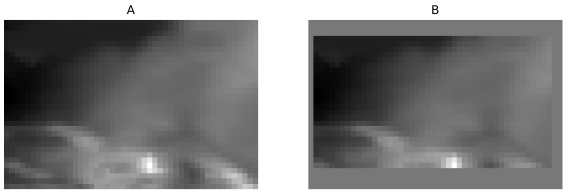
\includegraphics[scale=0.75]{figures/spatial_mapping.pdf}
    \caption{A: (32x48) Model input; B: (25x45) Mapped space}
    \label{fig:spatial_map}
\end{figure}
 